\documentclass[12pt]{article}
\usepackage{amssymb}
\usepackage{geometry}
\usepackage{amsmath, amsfonts, bm, graphicx}
\usepackage{float}
\geometry{margin=1in}
\title{}
\date{}
\author{}

\begin{document}

\section*{Mathematical Methods}

\begin{enumerate}
    \item Use the Taylor series expansion to find approximations. The ones for sin, cos, tan, and $(1 + x)^n$ are especially useful.
\begin{flalign*}
\sin x &= \sum_{n=0}^{\infty} (-1)^n \frac{x^{2n+1}}{(2n+1)!} 
       = x - \frac{x^3}{3!} + \frac{x^5}{5!} - \frac{x^7}{7!} + \cdots & \\[6pt]
\cos x &= \sum_{n=0}^{\infty} (-1)^n \frac{x^{2n}}{(2n)!} 
       = 1 - \frac{x^2}{2!} + \frac{x^4}{4!} - \frac{x^6}{6!} + \cdots & \\[6pt]
\tan x &= \sum_{n=1}^{\infty} \frac{B_{2n} (-4)^n (1-4^n)}{(2n)!}\,x^{2n-1} 
       = x + \frac{x^3}{3} + \frac{2x^5}{15} + \frac{17x^7}{315} + \cdots & \\[6pt]
(1+x)^m &= \sum_{n=0}^{\infty} \binom{m}{n} x^n 
       = 1 + mx + \frac{m(m-1)}{2}x^2 + \frac{m(m-1)(m-2)}{6}x^3 + \cdots &
\end{flalign*}
\underline{Note:} For small x, higher order terms reduce to zero

    \item Use complex exponentials to manipulate complicated trig functions.
\[
e^{ix} = \cos x + i \sin x
\]
    \item Solve differential equations by substituting in trial solutions. Especially you should recognize the differential equation for a simple harmonic oscillator and be able to come up with solutions to that ODE that satisfy any initial conditions you are given.

\[
\frac{d^2x}{dt^2} + \omega^2 x = 0
\]

\[
x(t) = A \cos(\omega t) + B \sin(\omega t)
\]
Wave equation: 
\[v^2 \frac{\partial ^2 y}{\partial x^2}=\frac{\partial^2 y}{\partial t^2}\]

\item Useful integration formulas:
\[\int\frac{1}{(x^2+a^2)^\frac{3}{2}}dx=\frac{x}{a^2\sqrt{x^2+a^2}}+C\]
\[\int\frac{x}{(x^2+a^2)^\frac{3}{2}}dx=-\frac{1}{\sqrt{x^2+a^2}}+C\]
\end{enumerate}
\newpage
\section*{Chapter 21 - Electric Charge}
\begin{enumerate}
    \item Explain what is electric charge, how you can tell if something carries an electric charge, how you could determine what the sign of the charge carriers is, and (qualitatively) how charge is transferred from one object to another.
    \begin{itemize}
        \item Electric charge is an intrinsic characteristic of the fundamental particles that make up matter. Electrically charged objects will exert electrostatic forces on each other (opposite charges attract and same charges repel).
        \item The elementary charge $e = 1.602 \times 10^{-19}C$
        \begin{itemize}
            \item Electrons has charge $-e$, protons has charge $+e$ and neutrons have no charge
        \end{itemize}
        \item Charges are transferred through direct contact and remain fixed once electrically isolated. It is possible to induce a charge on a conductor's surface via an external electric field moving its free electrons.
        \item To ground an object, set up a pathway of conductors between the object and the Earth (a big conductor/charge reservoir).
    \end{itemize}
    \noindent\underline{Note:} Charge is conserved when charges are transferred.
    \item Conductors and insulators:
    \begin{itemize}
        \item \textbf{Conductors:} Contain mobile/free electrons that can move freely within. If an excess charge is placed onto a conductor, it will spread over its surface. Thus, there is zero electric field within a conductor (always true, even with an external electric field, since non zero electric field will create current within the conductor).
        \item \textbf{Insulators:} Charges cannot move freely and is fixed after getting charged.
    \end{itemize}
    \item Use the Coulomb force law to solve mechanics problems involving electric charges.\\\\
    Charged particles exert forces on each other by:
    \[\vec{F}_{1\to2}=\frac{1}{4\pi\varepsilon_o}\frac{q_1q_2}{r^2}\hat{r}_{1\to2}\]
    Where
    \[\varepsilon_o=8.85 \times 10^{-12} \frac{C^2}{Nm^2} \quad \text{(Permittivity constant)}\]
    \[\vec{r}_{1\to2}=\left<\text{observation location}\right>-\left<\text{source location}\right>\]
\end{enumerate}
\newpage
\section*{Chapter 22 - Electric Fields}
\begin{enumerate}
    \item Define a field and identify whether a certain mathematical quantity is a field or not.\\\\
    Fields describe how a physical quantity varies throughout a region in space, with a value defined at every point in the region
    \begin{itemize}
        \item \textbf{Scalar fields:} assigns a scalar value to each point (Ex: temperature fields)
        \item \textbf{Vector fields:} assigns a vector (magnitude and direction) to each point (Ex: electric field)
    \end{itemize}    
    \item Electric field lines and the electric field are related by:
    \begin{itemize}
        \item The direction of the electric field at a point is tangent along the electric field line
        \item The magnitude of the electric field is proportional to the number of field lines per unit area in a plane perpendicular to the lines
    \end{itemize}
    \underline{Note:} The direction of $\vec{E}$ is the direction of the force that acts on a \textbf{positive test charge} (negative charges will accelerate antiparallel to the electric field lines)
\begin{figure}[H]
    \centering
    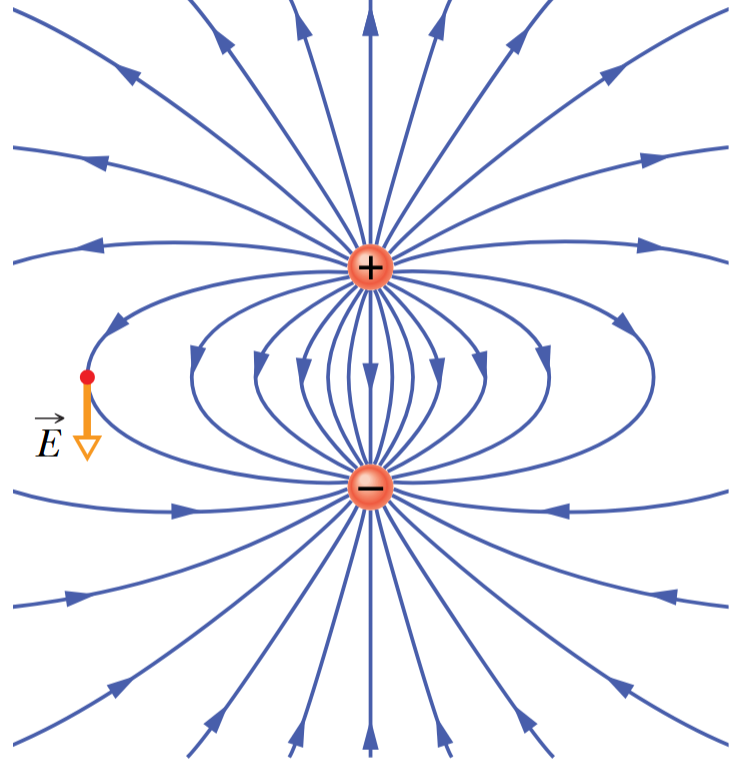
\includegraphics[width=0.3\textwidth]{e field dipole.png}
    \hspace{0.05\textwidth}
    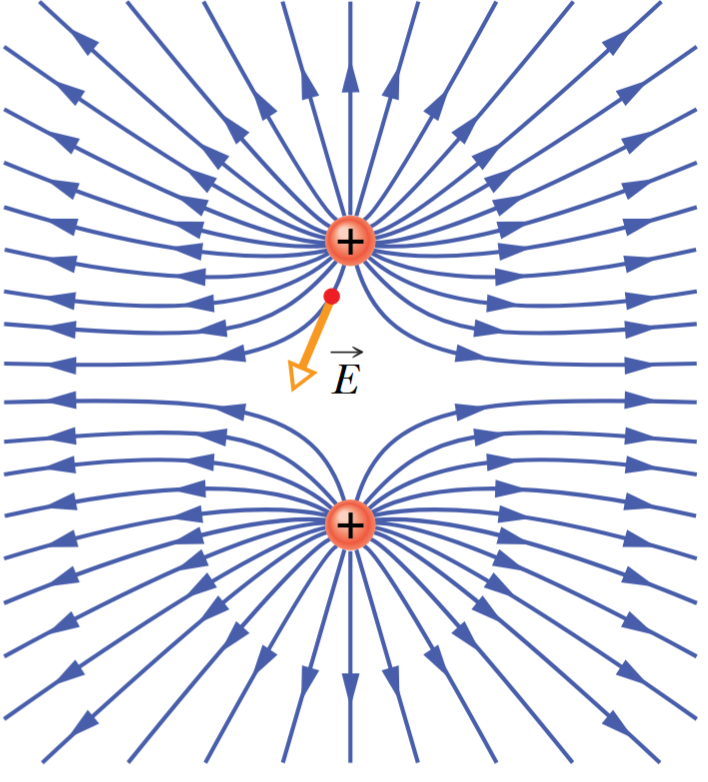
\includegraphics[width=0.3\textwidth]{e field same charge.png}
\end{figure}
    \item Given an electric field, find the force on a charged object.\\\\
    Force at point P on an object with charge $q_o$:
    \[\vec{F}_P=\vec{E}_Pq_o\]
    \item Find the electric field at any given location for a set of discrete charges.\\\\
    Electric field from a point charge q:
    \[\vec{E}=\frac{\vec{F}}{q_o}=\frac{1}{4\pi\varepsilon_o}\frac{q}{r^2}\hat{r}\]
    \item Find the electric field at any given location for a continuous charge distribution. In particular, be able to set up a complete integral for a higher (2 or 3) dimensional object that can be solved to obtain the electric field at a certain location by stacking up simpler (0 or 1) dimensional objects. Be able to solve the integrals for simple cases. Alternatively, use double or triple integrals to perform the same task.
    \begin{itemize}
        \item \textbf{Electric field from a line of charge:}
        \begin{figure}[H]
            \centering
            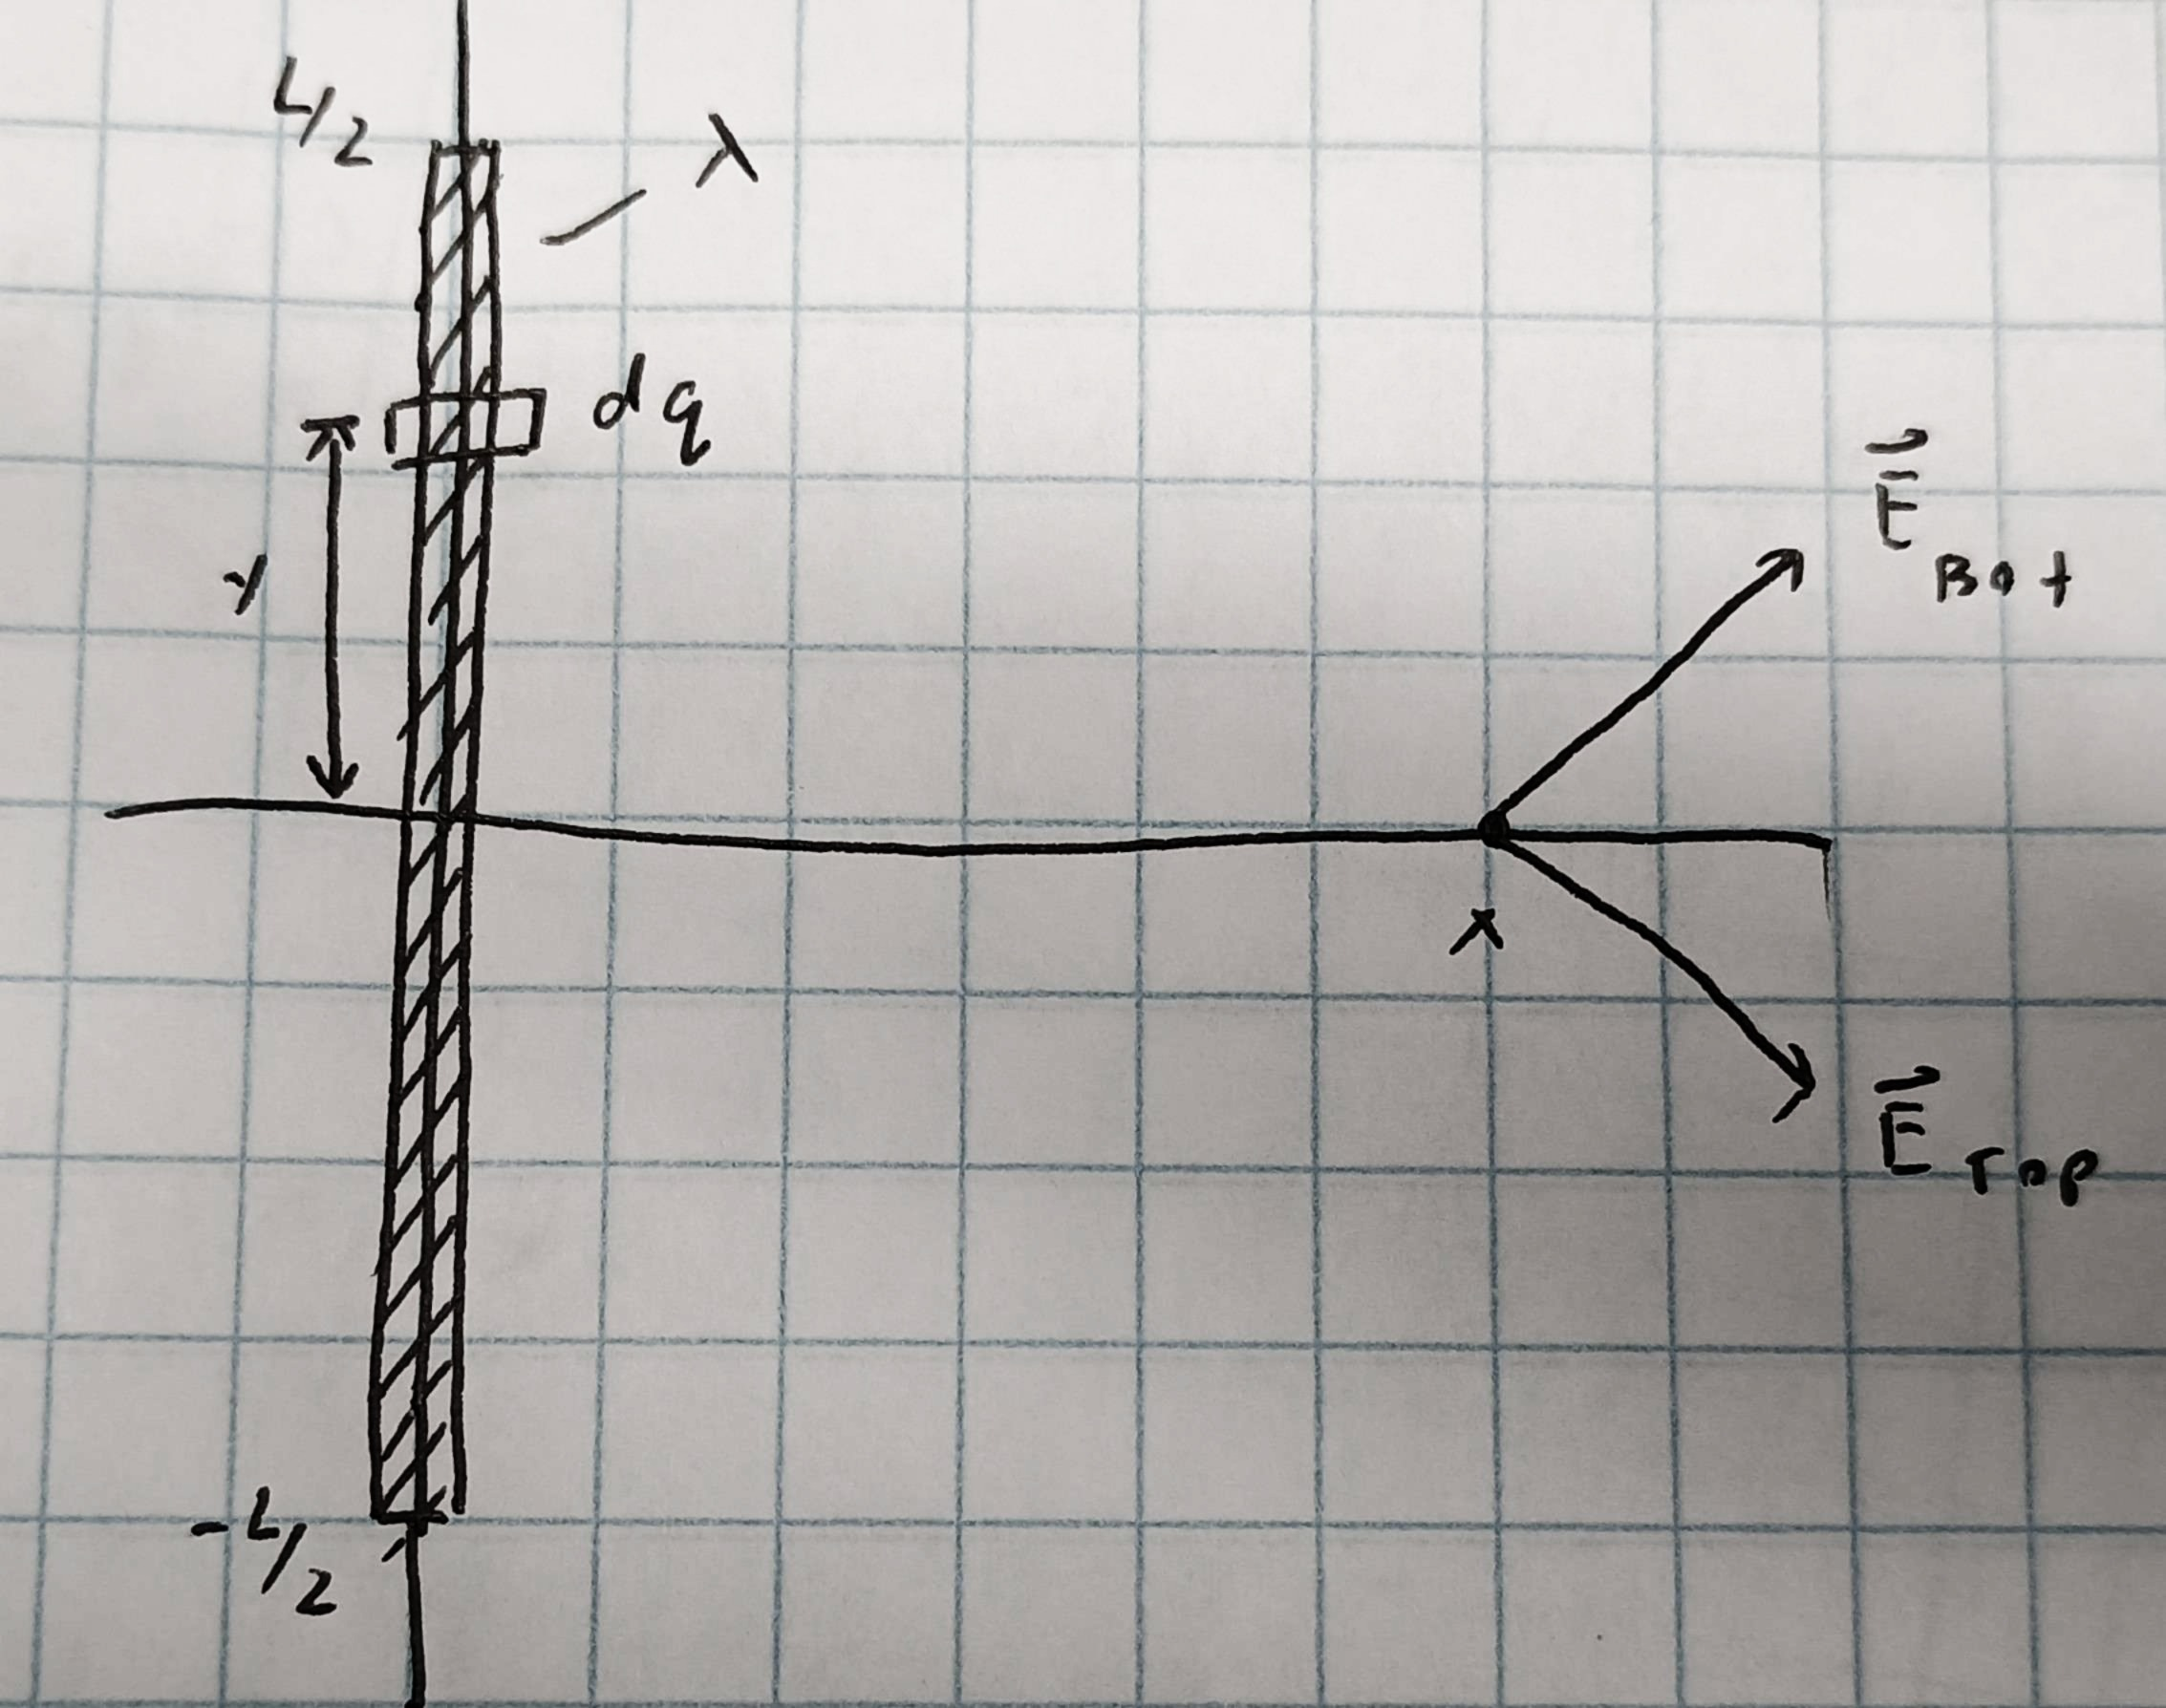
\includegraphics[width=0.4\textwidth]{line.jpg}
        \end{figure}
        Given:
        \begin{itemize}
            \item Total charge: $Q$
            \item Linear charge density $\lambda$
        \end{itemize}
        Calculating electric field from dq:
\[d\vec{E}=\frac{1}{4\pi\varepsilon_o}\frac{dq}{r^2}\hat{r}\]
\[\vec{r}=\left<x,0\right>-\left<0,y\right>=\left<x,-y\right>\]
\[\hat{r}=\frac{\left<x,-y\right>}{\sqrt{x^2+y^2}}\]
\[dq=\lambda dy=\frac{Q}{L}dy \quad \left(\lambda=\frac{Q}{L}\right)\]
\[\implies \int d\vec{E}=\int_{-L/2}^{L/2}\frac{1}{4\pi\varepsilon_o}\left(\frac{Q}{L}\right)\left(\frac{dy}{(x^2+y^2)^{3/2}}\right)\left<x,-y\right>\]
By symmetry, the components of the electric field in the y cancel out so
\[E_x=\frac{1}{4\pi\varepsilon_o}\left(\frac{Q}{L}\right)\int_{-L/2}^{L/2}\frac{x}{(x^2+y^2)^{3/2}}dy\]
\[\boxed{E_x = \frac{1}{4\pi\varepsilon_o} \left( \frac{1}{x\sqrt{x^2+(L/2)^2}} \right)}\]
        \item \textbf{Electric field from a ring of charge:} 
        \begin{figure}[H]
            \centering
            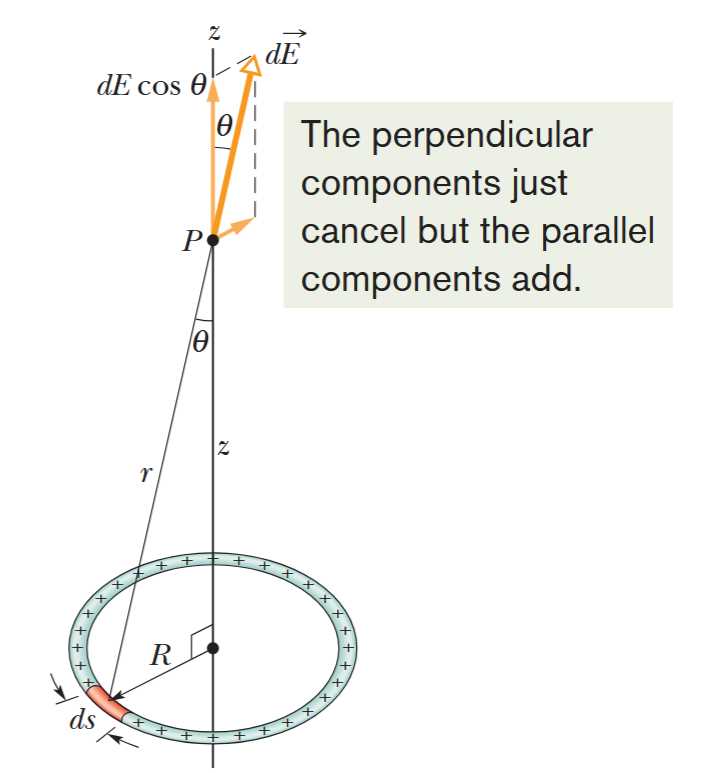
\includegraphics[width=0.4\textwidth]{ring.png}
        \end{figure}
        Given:
        \begin{itemize}
            \item Total charge: $Q$
            \item Linear charge density $\lambda$
            \item Ring radius $R$
        \end{itemize}
Calculating electric field from dq:
\[d\vec{E}=\frac{1}{4\pi\varepsilon_o}\frac{dq}{r^2}\hat{r}\]
\[\vec{r}=\left<0,0,z\right>-\left<Rcos\theta,Rsin\theta,0\right>=\left<-Rcos\theta,-Rsin\theta,z\right>\]
\[\hat{r}=\frac{\left<-Rcos\theta,-Rsin\theta,z\right>}{\sqrt{R^2+z^2}}\]
\[dq=\lambda ds=\frac{Q}{2\pi R}ds \quad \left(\lambda=\frac{Q}{2\pi R}\right)\]
\[\implies \int d\vec{E}=\int_{0}^{2\pi R}\frac{1}{4\pi\varepsilon_o}\left(\frac{Q}{2\pi R}\right)\left(\frac{ds}{(R^2+z^2)^{3/2}}\right)\left<-Rcos\theta,-Rsin\theta,z\right>\]
By symmetry, the components of the electric field in the radial directions cancel out so
\[E_z=\frac{1}{4\pi\varepsilon_o}\left(\frac{Q}{2\pi R}\right)\int_{0}^{2\pi R}\frac{z}{(R^2+z^2)^{3/2}}ds\]
\[\boxed{E_z = \frac{1}{4\pi\varepsilon_o} \left( \frac{Qz}{(R^2+z^2)^{3/2}} \right)}\]
        \item \textbf{Electric field from a disk of charge:}
        \begin{figure}[H]
            \centering
            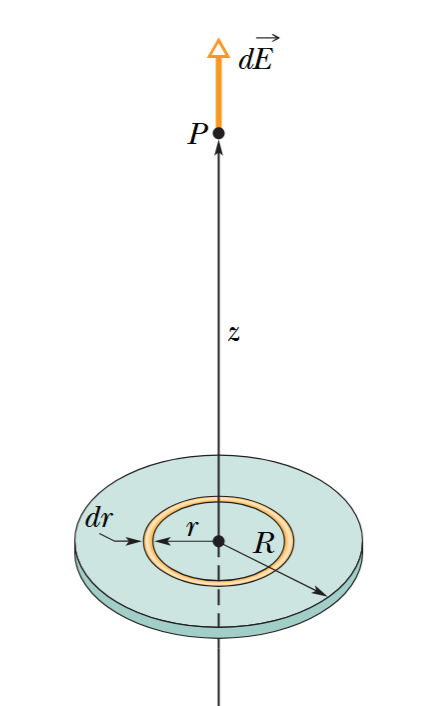
\includegraphics[width=0.3\textwidth]{disk.png}
        \end{figure}
        Given:
        \begin{itemize}
            \item Total charge: $Q$
            \item Surface charge density $\sigma$
            \item Disk radius $R$
        \end{itemize}
Using electric field from ring of radius r and charge q:
\[E_{ring,z} = \frac{1}{4\pi\varepsilon_o} \left( \frac{qz}{(r^2+z^2)^{3/2}} \right)\]
\[dE_{ring,z}=\frac{1}{4\pi\varepsilon_o} \left( \frac{zdq}{(r^2+z^2)^{3/2}} \right)\]
\[dq=\sigma dA =\left(\frac{Q}{\pi R^2}\right)\left(2\pi r dr\right)\]
\[\implies E_z=\int_{0}^{R}\frac{1}{4\pi\varepsilon_o}\left(\frac{Q}{\pi R^2}\right)\left(\frac{2\pi rz}{(r^2+z^2)^{3/2}}\right)dr\]
\[E_z=\frac{1}{4\pi\varepsilon_o}\left(\frac{2Q}{R^2}\right)\left(-\frac{z}{\sqrt{R^2+z^2}}--\frac{z}{\sqrt{z^2}}\right)\]
\[\boxed{E_z=\frac{1}{4\pi\varepsilon_o}\left(\frac{2Q}{R^2}\right)\left(1-\frac{z}{\sqrt{R^2+z^2}}\right)}\]
\newpage
        \item \textbf{Electric field from a sphere of charge:}
        \begin{figure}[H]
            \centering
            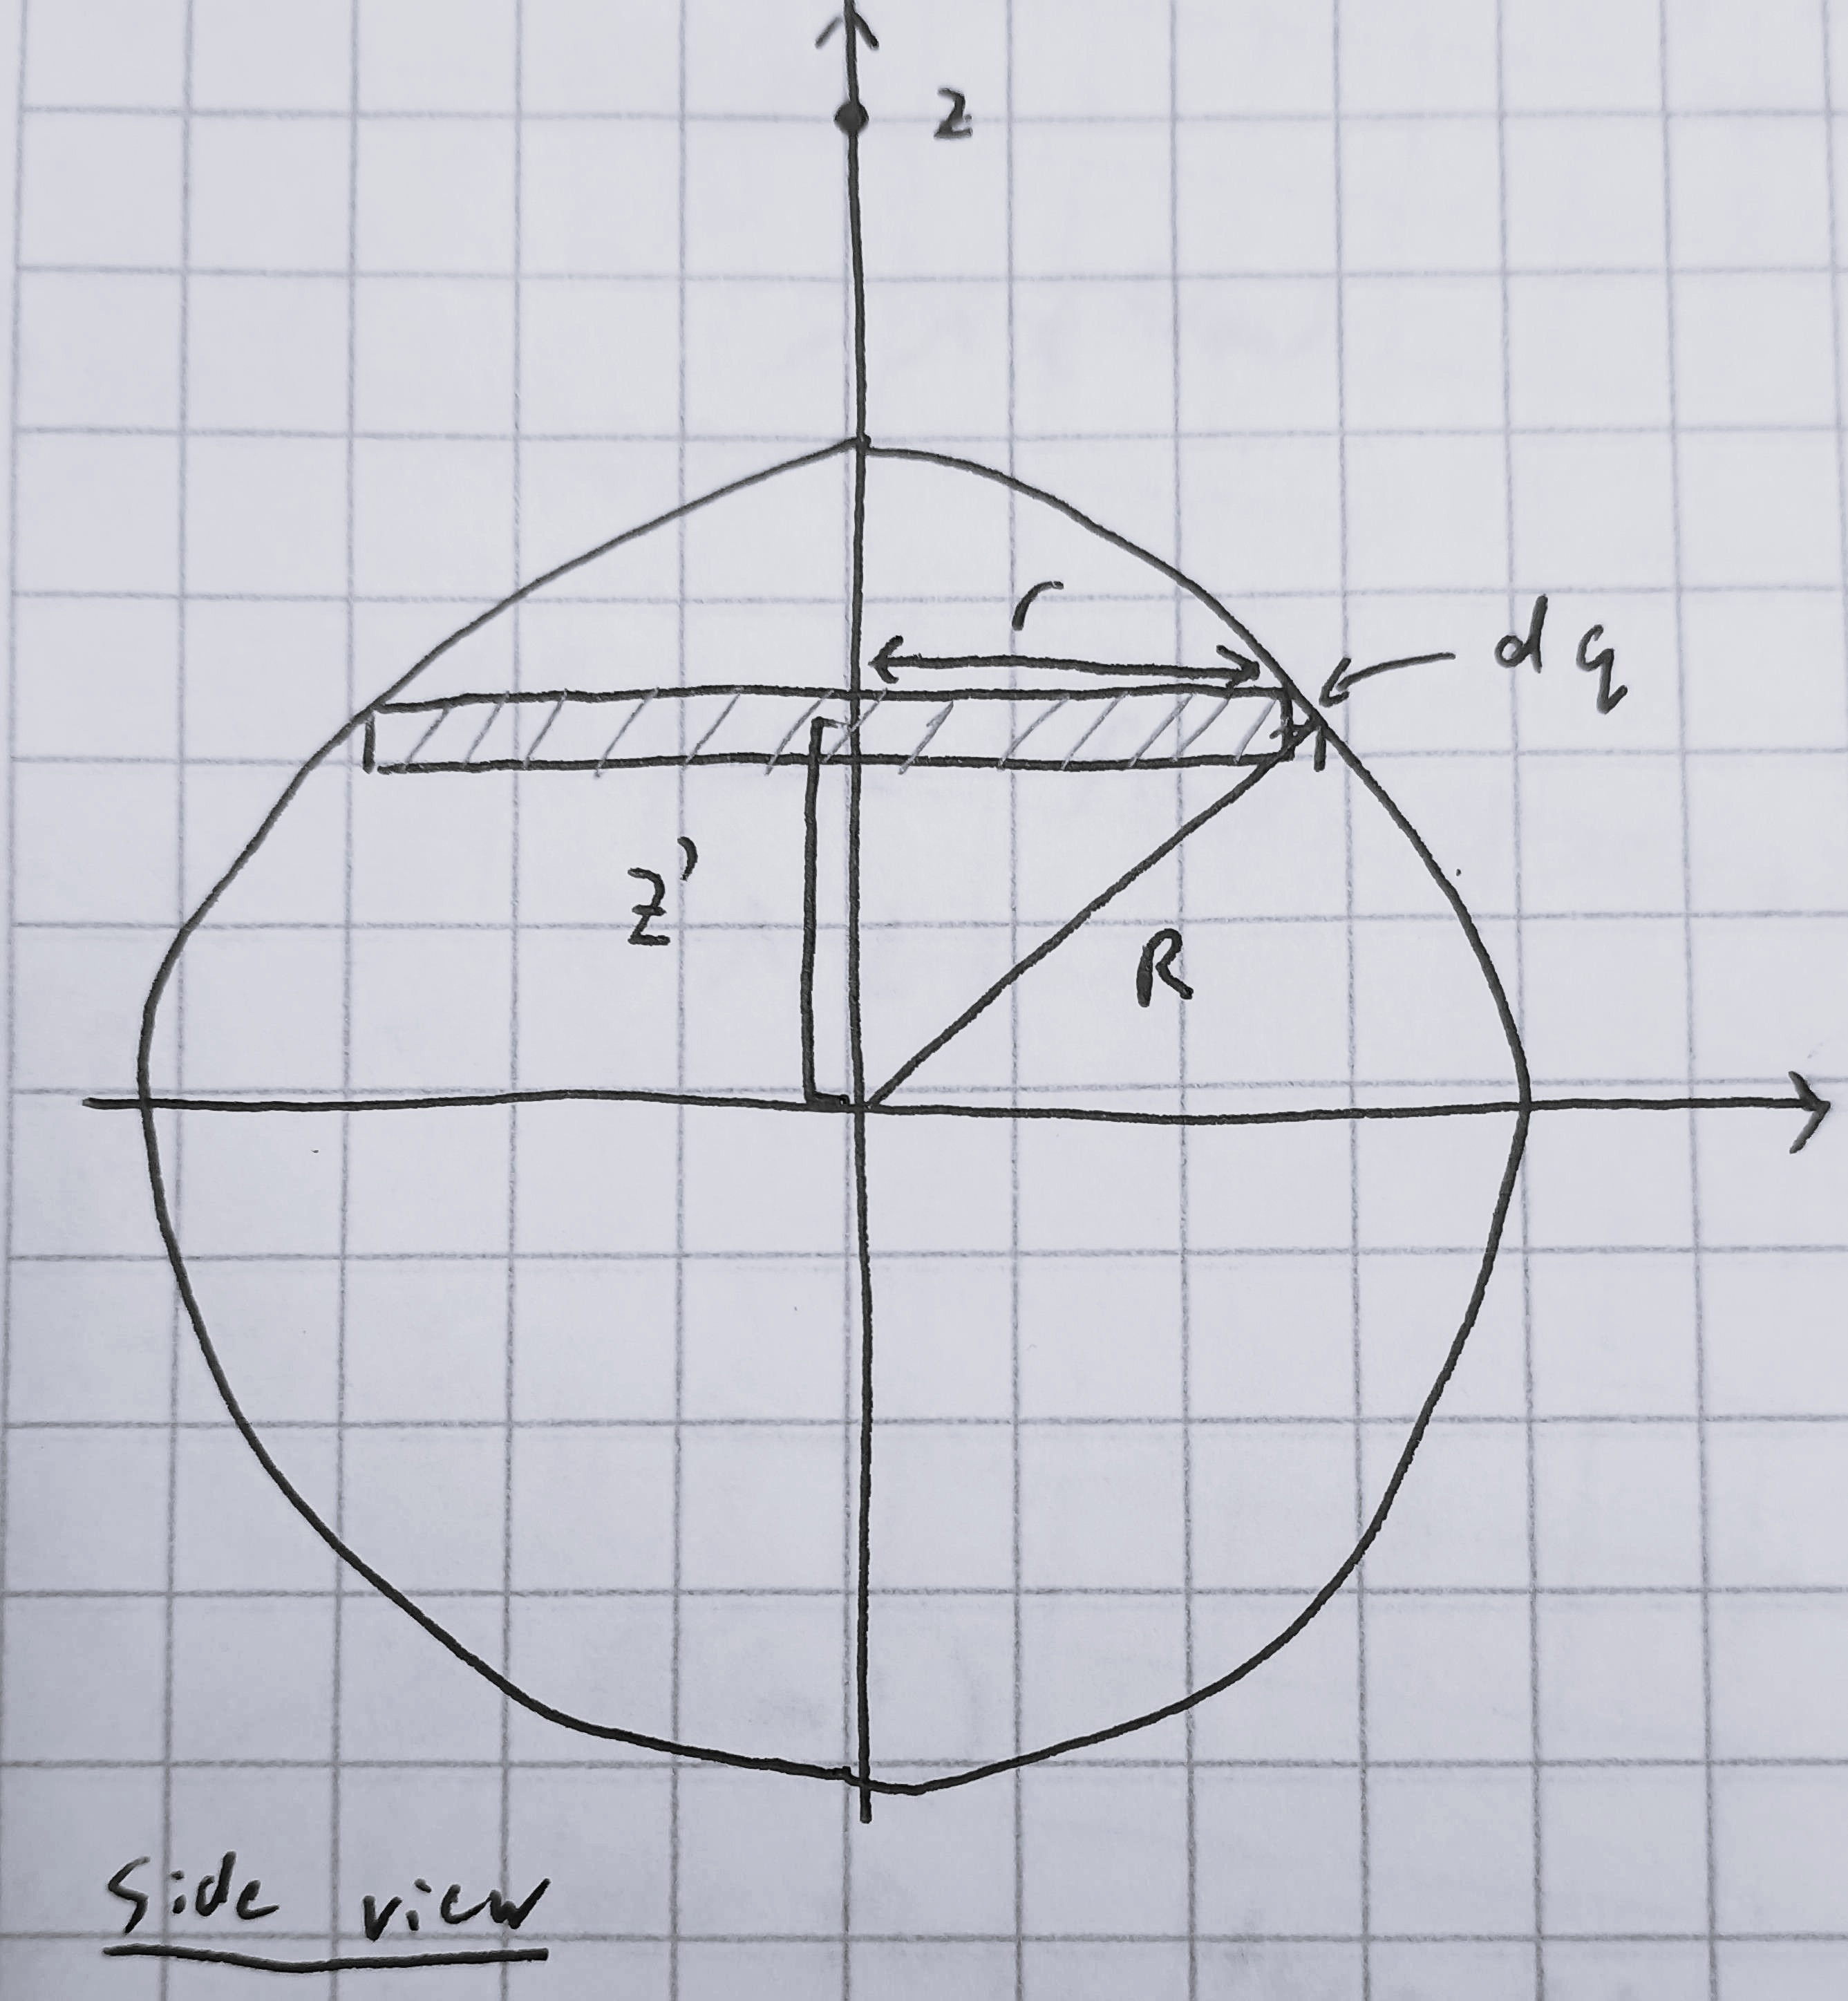
\includegraphics[width=0.3\textwidth]{sphere.jpg}
        \end{figure}
        Given:
        \begin{itemize}
            \item Total charge: $Q$
            \item Volume charge density $\rho$
            \item Sphere radius $R$
        \end{itemize}
Using electric field from disk of radius r and charge q, from a distance d away:
\[E_{disk,z}=\frac{1}{4\pi\varepsilon_o}\left(\frac{2q}{r^2}\right)\left(1-\frac{d}{\sqrt{r^2+d^2}}\right)\]
\[r=\sqrt{R^2-z'^2} \quad \text{(radius of disk as z' varies)}\]
\[d=z-z' \quad \text{(distance of disk from z as z' varies)}\]
\[dq_{disk}=\rho \pi r^2dz'=\left(\frac{Q}{\frac{4}{3}\pi R^3}\right)\pi r^2dz'\]
\[\implies E_{sphere,z}=\int_{-R}^{R}\frac{1}{4\pi\varepsilon_o}\left(\frac{2}{r^2}\right)\left(\frac{Q}{\frac{4}{3}\pi R^3}\right)\pi r^2dz'\left(1-\frac{d}{\sqrt{r^2+d^2}}\right)\]
Simplified and plugging in r and d:
\[E_{sphere,z}=\int_{-R}^{R}\frac{1}{4\pi\varepsilon_o}\left(\frac{2Q}{\frac{4}{3}\pi R^3}\right)\pi dz'\left(1-\frac{z-z'}{\sqrt{R^2-z'^2+(z-z')^2}}\right)\]

    \end{itemize}
    \item Find the force between objects that have continuous charge distributions, such as two lines of charge.
    \begin{itemize}
        \item Integrate to find the electric field from one continuous charge distribution at an observation point on the second continuous charge.
        \item Integrate again using the electric field on a charge dq on the second continuous charge for total force on it. (Ex: HW 6, Prob 1)
    \end{itemize}
    \item Find the torque and work done on an electric dipole by an electric field.\\\\
    The \textbf{Electric dipole moment ($\vec{P}=qd$)} points from the negative to the positive end of the dipole.
       \begin{figure}[H]
            \centering
            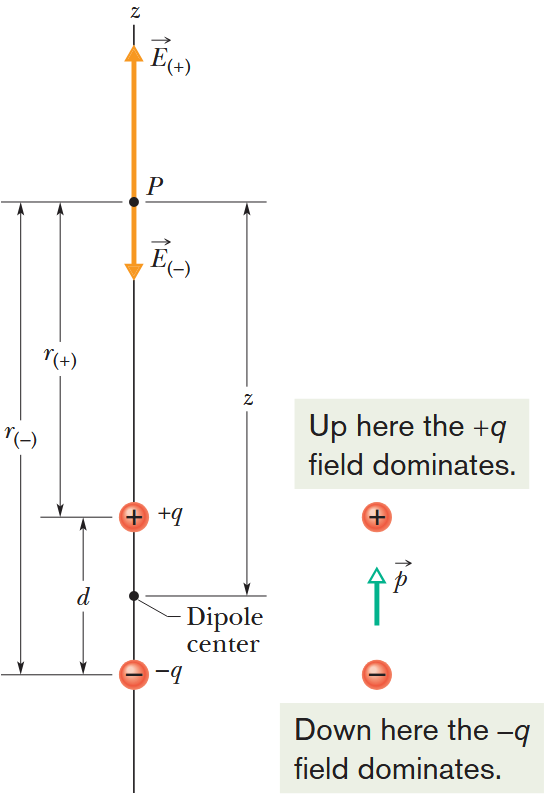
\includegraphics[width=0.3\textwidth]{Dipole moment.png}
        \end{figure}
    \begin{itemize}
        \item \textbf{Electric field due to an electric dipole}
\begin{flalign*}
\vec{E} &= \vec{E}_{+} + \vec{E}_{-} \\
        &= \frac{q}{4\pi\varepsilon_0}\left(\frac{1}{(z-d/2)^2}-\frac{1}{(z+d/2)^2}\right)
\end{flalign*}
Assuming $z>>d$
\[\boxed{\vec{E}=\frac{1}{4\pi\varepsilon_o}\frac{2qd}{z^3}}\]
\item \textbf{Torque on a dipole in an electric field}
   \begin{figure}[H]
            \centering
            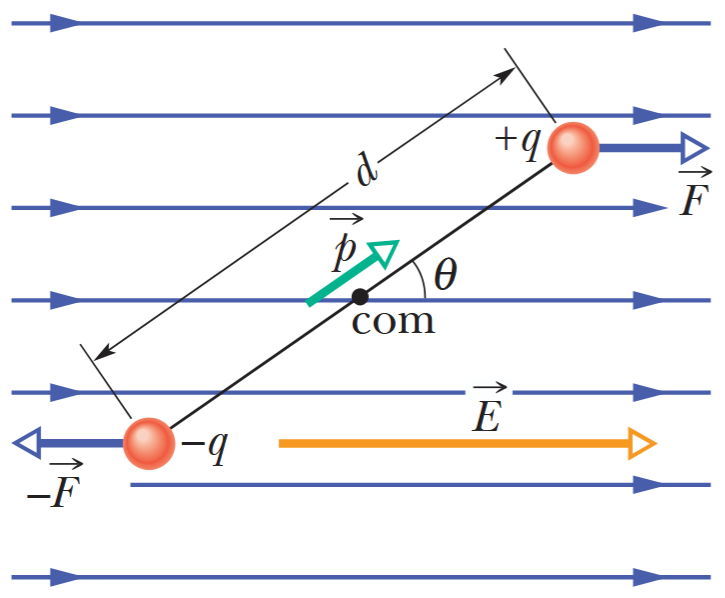
\includegraphics[width=0.3\textwidth]{Dipole torque.png}
    \end{figure}
    In a uniform electric field, the electrostatics on the charged ends of the dipole are equal and opposite, thus there is zero net force and the center of mass does not move.\\\\
    However, there is non-zero torque:
    \[\tau=pEsin\theta\]
    \[\boxed{\vec{\tau}=\vec{p}\times\vec{E}}\]
\item \textbf{Potential energy of an electric dipole}
\begin{itemize}
    \item Define the zero potential energy as when $\theta=90^\circ$
    \item We can find the potential energy at any $\theta$ by calculating the work done by the field when the dipole is rotated from $\theta$ to $90^\circ$.
    \[\Delta U=-W_c\]
    \[U=-\int_{90^\circ}^{\theta}\tau d\theta=-\int_{90^\circ}^{\theta} pEsin\theta d\theta\]
    \[U=-pEcos\theta\]
    \[\boxed{U=-\vec{p}\cdot\vec{E}}\]
\end{itemize}
The dipole has the least potential energy at equilibrium where $\vec{p}$ and $\vec{E}$ are lined up and $\vec{\tau}=\vec{p}\times\vec{E}=0$. It is like a pendulum where it requires work to rotate the dipole to any other orientation.
    \end{itemize}
  
    
\end{enumerate}

\section*{Chapter 23 - Gauss's Law}
\begin{enumerate}
    \item Explain Gauss's law and how it relates electric charge to electric flux.\\\\
Gauss’s law can be applied to find the electric field produced by a symmetric charge distribution (Ex: spherical, cylindrical, or planar symmetry). When other non-symmetric charges are also present, Gauss’s law can still be used separately to find the field due to the symmetric charge alone.
This is because charges located outside the chosen Gaussian surface contribute no net flux through that surface (the field lines from external charges enter and exit equally) and therefore do not appear in the flux integral.
The total electric field at a point is then obtained by superposition of the symmetric field (found via Gauss’s law) and the field from the external or asymmetric charges (found using Coulomb’s law or direct integration).\\\\
\textbf{Gauss's Law}
where $d\vec{A}$ is an infinitesimal area element whose direction is normal to the surface.
\[\boxed{\oint \vec{E} \cdot d\vec{A} = \frac{Q_{\text{enc}}}{\varepsilon_0} \quad \text{Integral form}}\]
\[\boxed{\vec{\nabla} \cdot \vec{E} = \frac{\rho}{\varepsilon_o} \quad \text{Differential form (local version)}}\]
    \item Given an electric field and a surface, calculate the flux of the electric field through the surface.\\\\
The electric flux through a surface $S$ is defined as
\[\Phi_E = \iint_S \vec{E} \cdot d\vec{A}\]


For a uniform electric field $\vec{E}$ and a flat surface of area $A$, the flux simplifies to
\[
\Phi_E = EA \cos\theta,
\]
where $\theta$ is the angle between $\vec{E}$ and the surface normal.
    \item Explain the conditions necessary in order to use Gauss's law to solve for an electric field. Identify geometries for which Gauss's law can be used or for which the electric field must be found using Coulomb's law. For applicable cases, construct an appropriate Gaussian surface and determine the electric field using Gauss's law.\\\\
    We can find the electric field using Gauss's law if we can pick a Gaussian surface such that:
    \begin{itemize}
        \item The electric field is constant over the surface
        \item The electric field is parallel or normal to the surface everywhere
    \end{itemize}
\textbf{Symmetries and its respective Gaussian surfaces}
\begin{itemize}
    \item \textbf{Spherical}
    \[Q_{enc}=\rho V=\frac{4}{3}\rho \pi r^3\]
    \[\text{(Surface Area)}=4\pi r^2\]
    \item \textbf{Cylindrical}\\
    Ex: Infinite line of charge (Gaussian cylinder)
\[Q_{enc}=\lambda L\]
\[\text{(Surface Area with non-zero flux)}=2\pi r L\]
\underline{Note:} The electric field is radial and there is zero flux through the caps.
    \item \textbf{Planer}\\
    Ex: Infinite sheet of charge (Gaussian cylinder)
    \[Q_{enc}=\sigma A=\sigma \pi r^2\]
    \[\text{(Surface Area with non-zero flux)}=2\pi r^2\]
    \underline{Note:} The electric field is normal and there is zero flux through the sleeve of the cylinder.
\end{itemize}
    \item Use Gauss's law to derive the properties of electric fields in and around conductors. State any required conditions for the standard properties to apply.\\\\
\textbf{Properties of Conductors:}
\begin{itemize}
    \item There is zero electric field inside a conductor (in equilibrium).
    \item The electric field near the surface of a conductor is always normal with magnitude
    \[\vec{E}=\frac{\sigma}{\varepsilon_o}\]
    \item A conductor only has excess charge on its surface.
\end{itemize}
    \item Given an electric field as a function of position, find the charge density.\\\\
    Ex: A insulating spherical charge with and varying charge density $\rho (r)=$ produces an electric field $\vec{E}=Kr^4$
    \begin{flalign*}
    \oint \vec{E} \cdot d\vec{A} =& \frac{Q_{\text{enc}}}{\varepsilon_0}\\
    =&\frac{1}{\varepsilon_o}\int\rho (r)\;dV\\
    =&\frac{1}{\varepsilon_o}\int_{0}^{r_o}\rho (r) 4\pi r^2\;dr
    \end{flalign*}
    \[\vec{E}(r_o)(4\pi r_o^2)= \frac{1}{\varepsilon_o}\int_{0}^{r_o}\rho (r) 4\pi r^2\;dr\]
    \[\frac{d}{dr}\left(\vec{E}(r_o)(4\pi \varepsilon_o r_o^2)\right)= \rho (r_o) 4\pi r_o^2\]
    \[\frac{\varepsilon_o }{r_o^2}\frac{d}{dr}\left(Kr_o^4(r_o^2)\right)= \rho (r_o)\]
    \[\rho (r_o)=\frac{\varepsilon_o }{r_o^2}\left(6Kr_o^5\right)=6K\varepsilon_o r_o^3\]
\end{enumerate}
\newpage
\section*{Chapter 24 - Electric Potential}
\begin{enumerate}
    \item Define the electric potential, its relation to electric potential energy, and its relation to the electric field.
    \begin{itemize}
\item \textbf{Electric Potential}\\
The electric potential at a point in an electric field is:    
\[\boxed{V=\frac{U}{q}}\]
The potential difference between any two points in an electric field is:
\[\Delta V=\frac{\Delta U}{q}\]
Since the electrostatic force is a conservative force, it follows the relationship that $\Delta U = -W_{conservative}$
\[\boxed{\Delta V = \frac{-W}{q}}\]
If we define the potential energy to be zero at $\infty$ then the potential at any point is:
\[V=\frac{-W_{\infty}}{q}\]
Where $W_{\infty}$ is the work done by the electric field on a charged particle as it moves from $\infty$ to a point.
\item \textbf{Electric potential energy of a system of point charges}\\
The electric potential of a system of fixed point charges (at rest) is equal to the work that must be done by an external force to assemble the system, bringing in each charge from $\infty$.\\\\
\underline{Ex:}
   \begin{figure}[H]
            \centering
            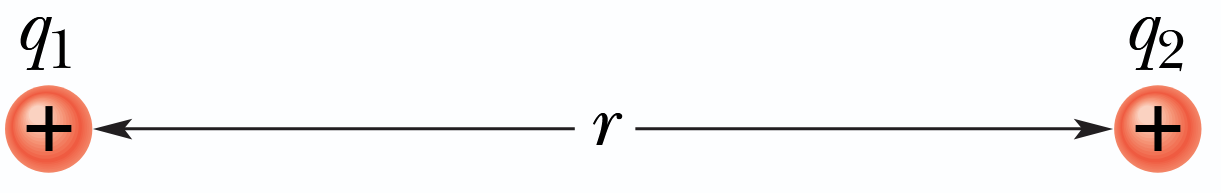
\includegraphics[width=0.4\textwidth]{energy 1.png}
    \end{figure}
\begin{itemize}
    \item First bring in $q_1$ from $\infty$: zero work is done because there is no electrostatic force on it, thus force applied is zero.
    \item Then bring in $q_2$ from $\infty$: there is an electric field from $q_1$
    \[W_{ext}=-W_{field}=q_2 \Delta V \quad (V_i =0)\]
    \[U=W_{ext}=q_2V_1=\frac{1}{4\pi\varepsilon_o}\frac{q_1q_2}{r}\]
\end{itemize} 
\underline{Ex:}
   \begin{figure}[H]
            \centering
            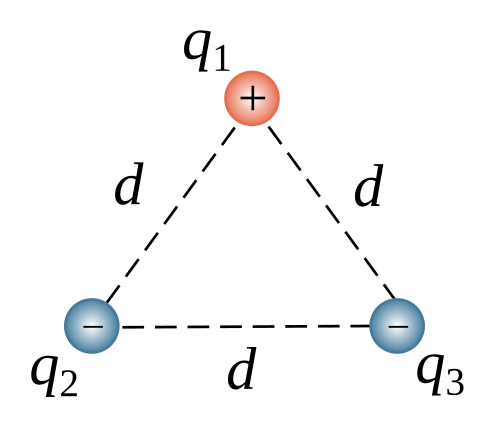
\includegraphics[width=0.3\textwidth]{energy2.png}
    \end{figure}
\begin{itemize}
    \item Zero work is done to bring in $q_1$
    \item Work done to bring in $q_2$ is due to potential from $q_1$
    \[U_{12}=\frac{1}{4\pi\varepsilon_o}\frac{q_1q_2}{d}\]
    \item Work done to bring in $q_3$ is due to the potential from BOTH $q_1$ and $q_2$
    \[U_{13}+U_{23}=\frac{1}{4\pi\varepsilon_o}\frac{q_1q_3}{d}+\frac{1}{4\pi\varepsilon_o}\frac{q_2q_3}{d}\]
    \[U=W_{ext}=U_{12}+U_{13}+U_{23}\]
    \underline{Note:} Order doesn't matter when it comes to assembling the system of charges.
\end{itemize} 
\item \textbf{Relationship Between Potential and the Electric Field}\\
Since the work done by the electrostatic force and potential is related by:
\[\Delta V = \frac{-W}{q}\]
Work can be calculated by:
\[dW=\vec{F}\cdot d\vec{s}=q\vec{E}\cdot d\vec{s}\]
\[W=q\int_{i}^{f}\vec{E}\cdot d\vec{s}\]
Thus,
\[\boxed{\Delta V=-\int_{i}^{f}\vec{E}\cdot d\vec{s}}\]
\textbf{To calculate the electric field given potential:}
\[\boxed{\vec{E}=-\vec{\nabla}V}\]
\underline{Note:}
\[\vec{\nabla} =
\frac{\partial}{\partial x}\,\hat{\imath}
+ \frac{\partial}{\partial y}\,\hat{\jmath}
+ \frac{\partial}{\partial z}\,\hat{k}\]
    \end{itemize}
    \item Given a distribution of charges determine the electric potential in two different ways by either (1) using a line integral and a given electric field or (2) building the potential up by summing discrete charges or integrating over a charge distribution.\\\\
    \textbf{Method 1:} Integrate from $\infty$ to observation point\\
    \[\Delta V=-\int_{i}^{f}\vec{E}\cdot d\vec{s}\]
    \underline{Potential of a point charge}
       \begin{figure}[H]
            \centering
            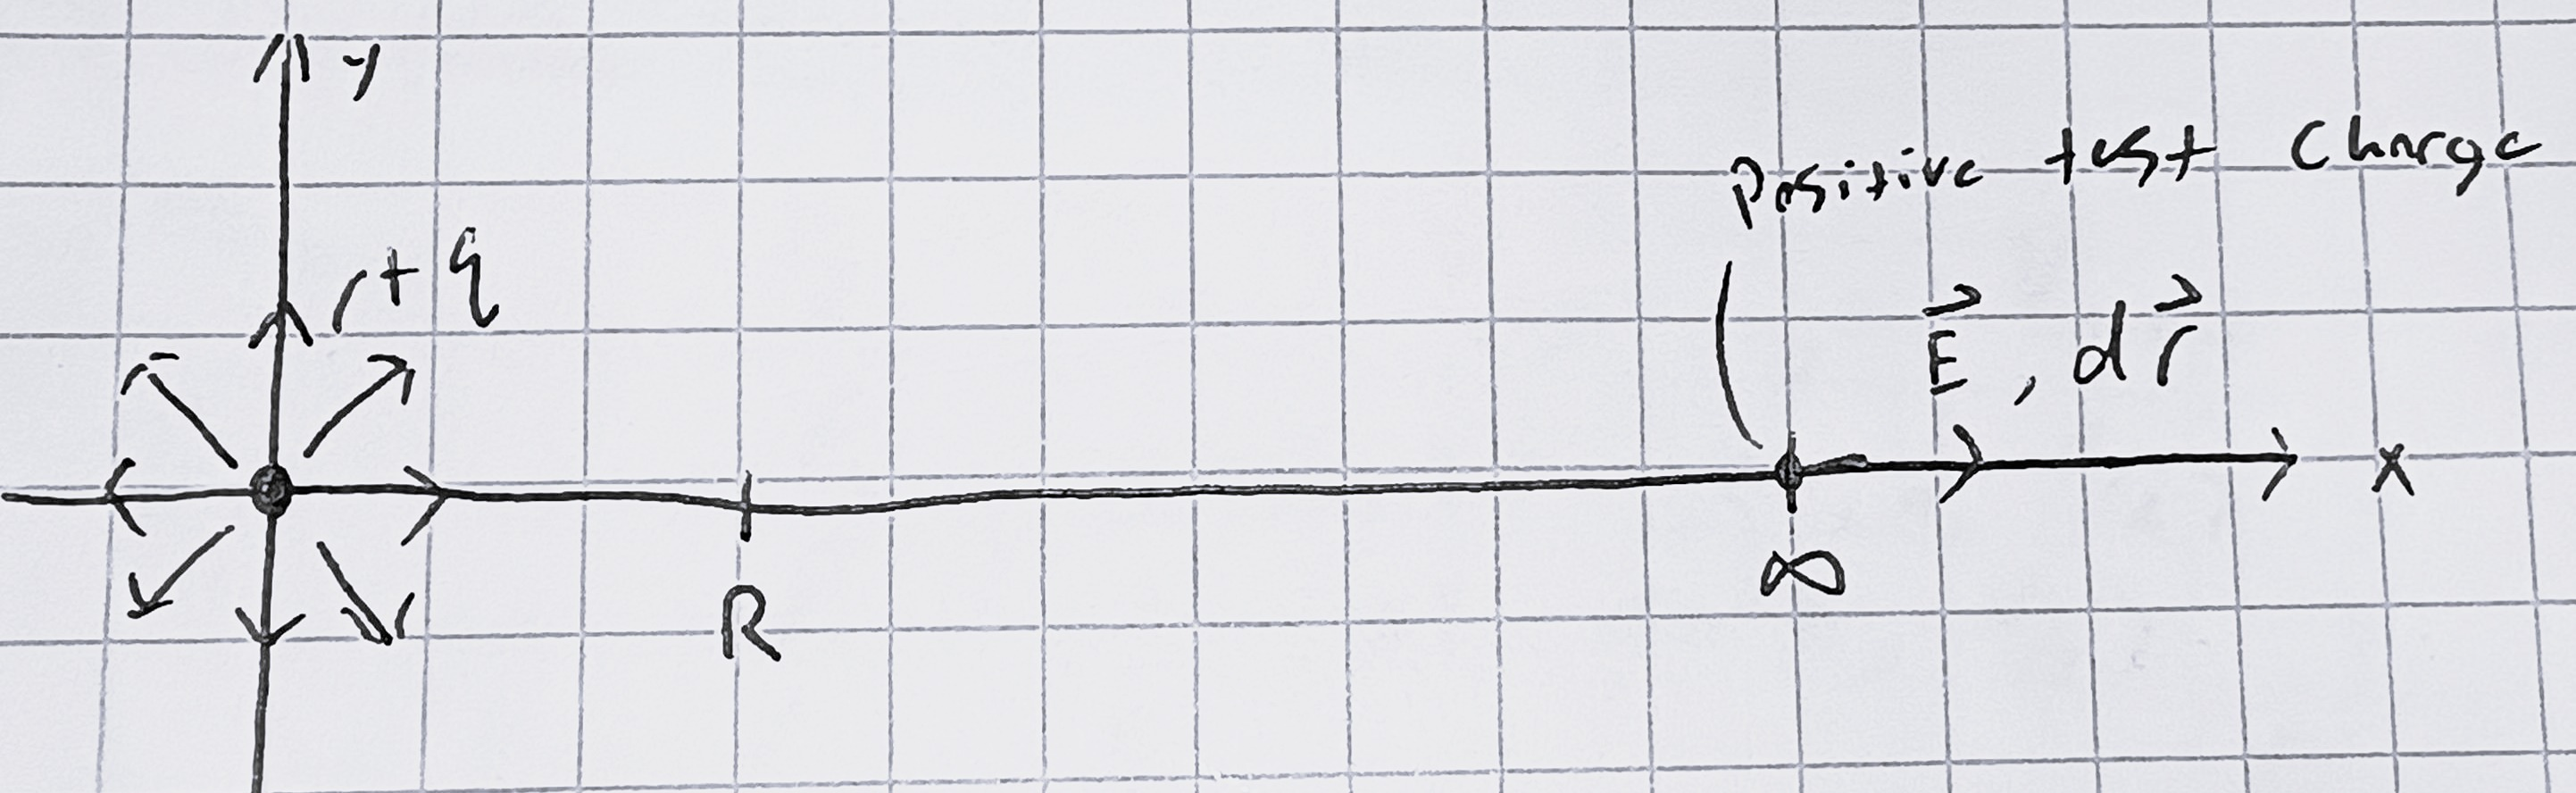
\includegraphics[width=0.7\textwidth]{point.JPG}
    \end{figure}
    We will move a positive test charge from $\infty$ to $R$ towards a point charge.
    \[V_f-V_i=-\int_{R}^{\infty}\vec{E}\cdot d\vec{r} \quad (V(\infty)=0)\]
    \begin{align*}
        V(R)=&-\int_{\infty}^{R}\frac{1}{4\pi\varepsilon_o}\frac{q}{r^2}\hat{r}\cdot d\vec{r}\quad (\hat{r}\cdot d\vec{r}=dr)\\
        =&-\frac{q}{4\pi\varepsilon_o}\int_{\infty}^{R}\frac{1}{r^2}dr\\
        =&-\frac{q}{4\pi\varepsilon_o}\left(\frac{-1}{r}\right) \bigg|_{\infty}^{R}
    \end{align*}
    \[\boxed{V=\frac{q}{4\pi\varepsilon_o r}\quad \text{(point charge)}}\]
    \underline{Note:} $d\vec{r}$ points in the same direction as the coordinate axes, the direction of the particle's motion comes from the integration bounds.\\\\
    Generally, this method is used when we can easily find the electric field.\\\\
    \textbf{Method 2:} Integrating $dV$ from discrete point charges.\\
    Using the potential from a point charge:
    \[V=\frac{q}{4\pi\varepsilon_o r}\implies dV=\frac{dq}{4\pi\varepsilon_o r}\]
    \[\boxed{V=\frac{1}{4\pi\varepsilon_o}\int \frac{dq}{r}}\]
    \item Know and use the properties of the potential for conductors.\\\\
    \textbf{Conductors are equipotential volumes}\\
    The potential at every point within an equipotential surface/volume is EQUAL. Thus, no work is done by an electric field on a charge as it moves through an equipotential ($\Delta V=0 \implies W=0$).
    \begin{figure}[H]
            \centering
            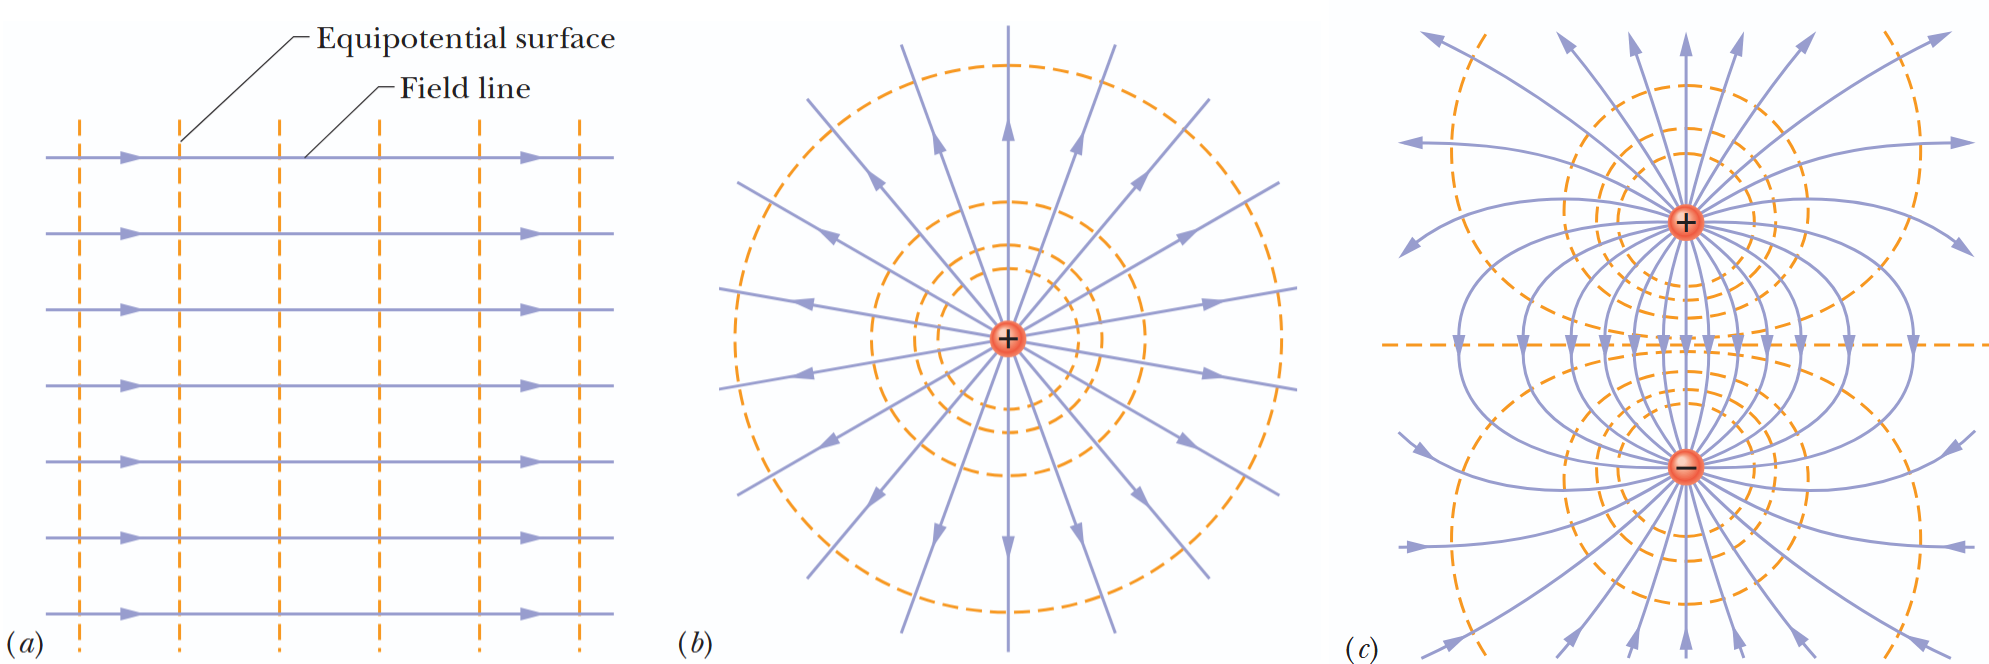
\includegraphics[width=0.9\textwidth]{equipotential.png}
    \end{figure}
    \underline{Note:} Equipotential surfaces are always perpendicular to the electric field ($\vec{E}\cdot d\vec{s}=0$)\\\\
    \underline{Ex:} Two conducting spheres are connected with a wire. Initially, sphere 1 is charged with $Q_1=Q$ and sphere 2 is neutral. How much charge ends up on each sphere after the connection?
    \begin{figure}[H]
            \centering
            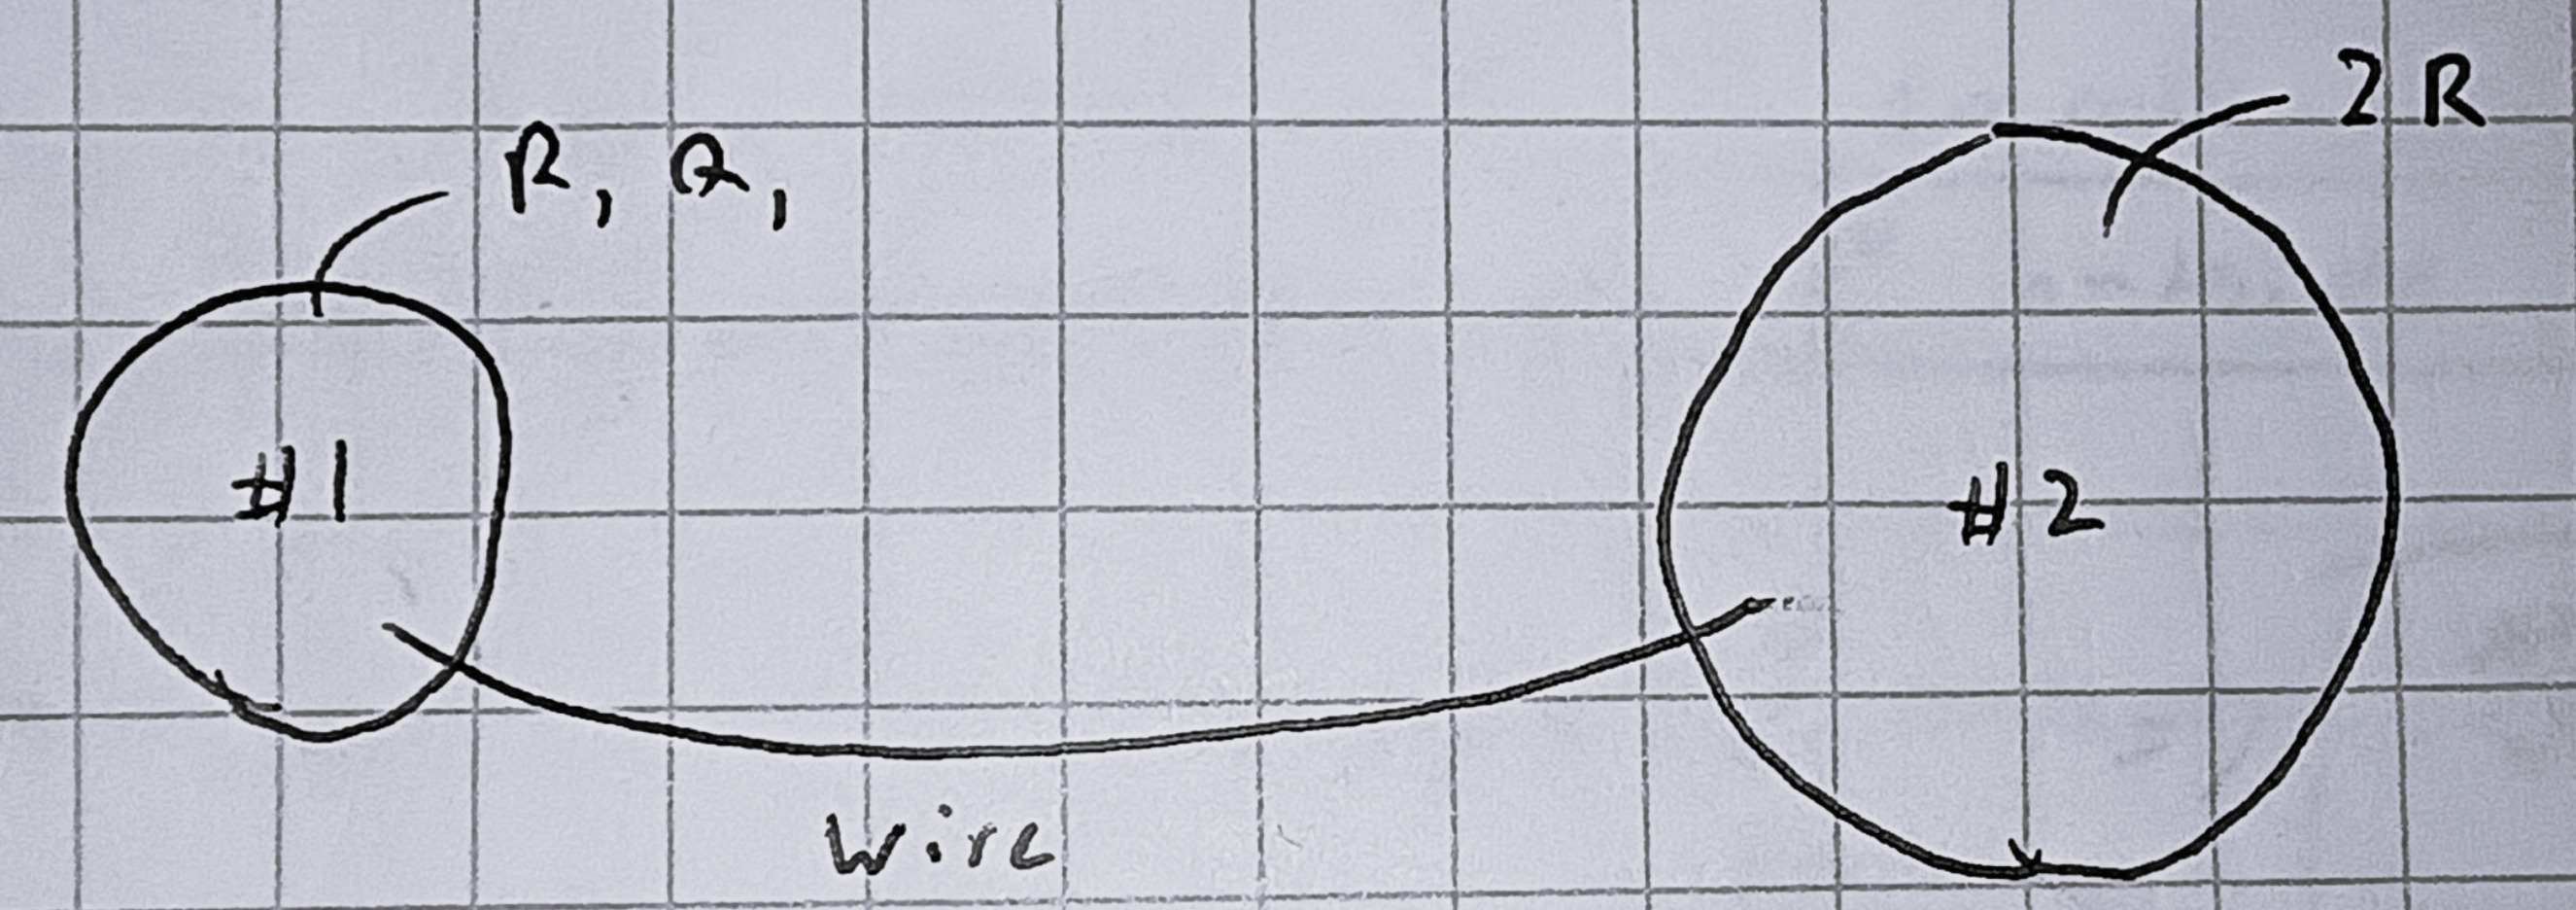
\includegraphics[width=0.5\textwidth]{conductingsphere.JPG}
    \end{figure}
    \[V_{sphere}=\frac{1}{4\pi\varepsilon_o}\frac{q}{r}\]
    Since there is no potential difference between the two spheres $V_1=V_2$
    \[\frac{1}{4\pi\varepsilon_o}\frac{Q_1}{R}=\frac{1}{4\pi\varepsilon_o}\frac{Q_2}{2R}\]
    \[\implies Q_1=\frac{Q_2}{2}\]
    Since the total charge is conserved
    \[Q_1+Q_2=Q\]
    \[\implies Q_1=\frac{Q}{3},\quad Q_2=\frac{2Q}{3}\]
    \textbf{Finding the charge distribution on the surface of a conducting sphere}\\
    Suppose a charged conducting sphere with radius R and surface charge density $\sigma$
    \[\int \vec{E}\cdot\hat{n}dA=\frac{Q_{enc}}{\varepsilon_o}\]
    \[E(4\pi r^2)=\frac{4\pi R^2 \sigma}{\varepsilon_o}\]
    \[E(r)=\frac{\sigma R^2}{\varepsilon_o r^2}\]
    \[V=-\int_{\infty}^{R}\frac{\sigma}{\varepsilon_o}\frac{R^2}{r^2}dr\]
    Thus the potential at the surface of a conducting sphere:
    \[V=\frac{\sigma R}{\varepsilon_o}\]
    Consider the following conductor:
        \begin{figure}[H]
            \centering
            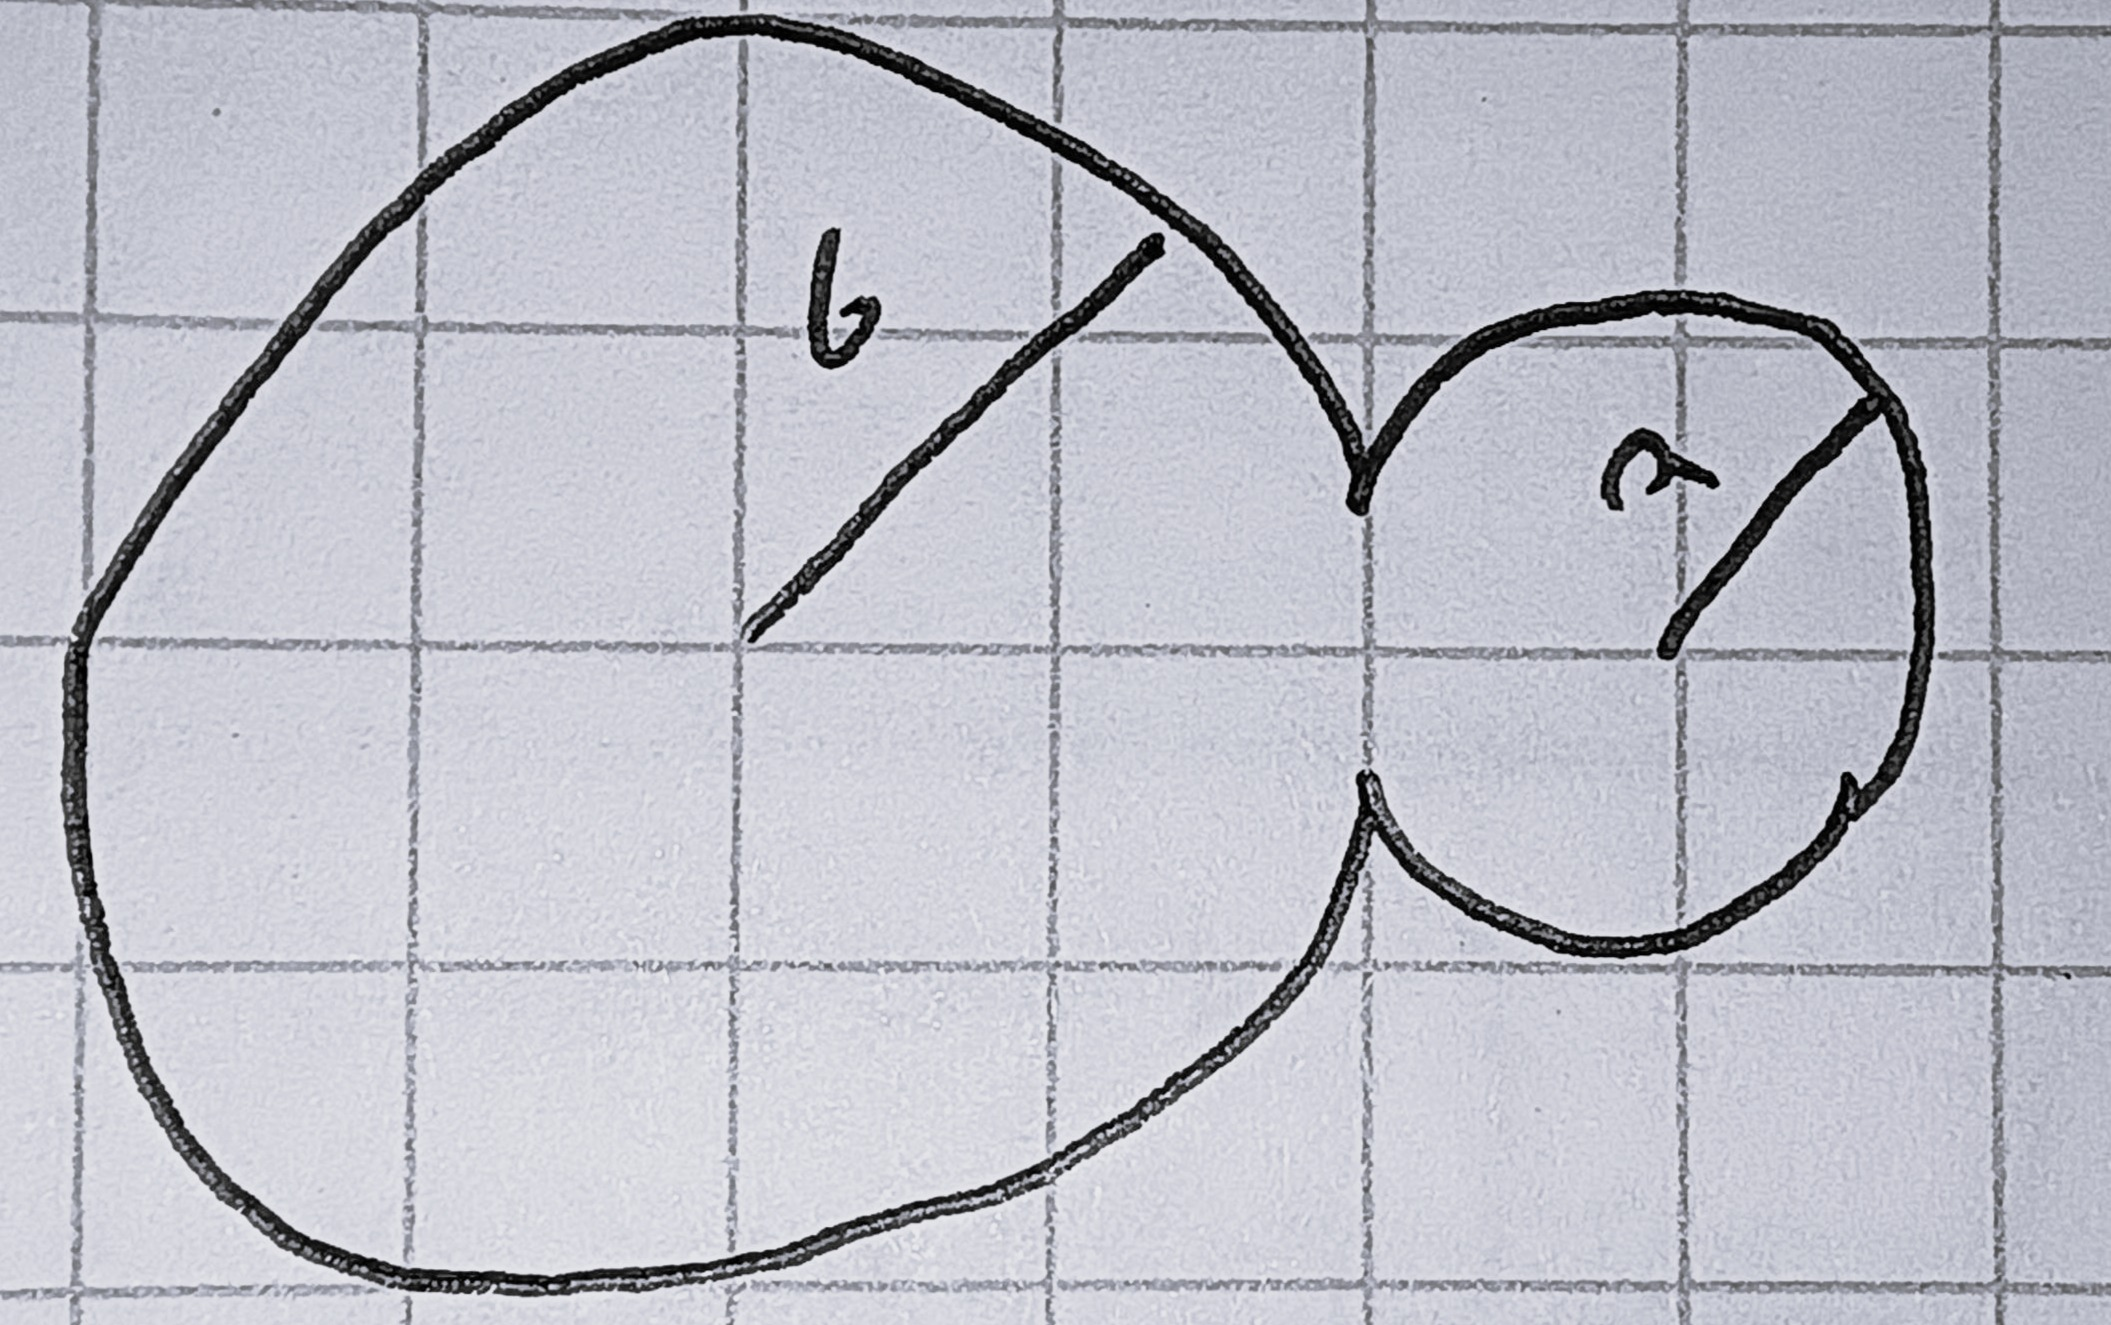
\includegraphics[width=0.5\textwidth]{distribution.JPG}
    \end{figure}
    Since we know the potential across the surface is equal, and that each blob is approx a sphere:
    \[V=\frac{\sigma_a a}{\varepsilon_o}=\frac{\sigma_b b}{\varepsilon_o}\]
    Thus, $\sigma_b > \sigma_a$ since $b>a$. In other words, charges concentrate when the radius of curvature is small (ie. pointy)
\newpage
    \item Use the ``method of images'' to find the potential for a charge suspended over a grounded infinite conducting plate.\\\\
    From the differential form of Gauss's Law:
    \[\vec{\nabla} \cdot \vec{E} = \frac{\rho}{\varepsilon_o}\]
    \[\vec{\nabla} \cdot (-\vec{\nabla}V) = \frac{\rho}{\varepsilon_o} \quad (\vec{E}=-\vec{\nabla}V)\]
    \[\boxed{-\nabla^2 V = \frac{\rho}{\varepsilon_o} \quad \text{(Poisson's Equation)}}\]
    When $\rho=0$
    \[\boxed{\nabla^2 V = 0 \quad \text{(Laplace's Equation)}}\]
Where 
\[\nabla^2 = 
\frac{\partial^2}{\partial x^2} +
\frac{\partial^2}{\partial y^2} +
\frac{\partial^2}{\partial z^2}\]
We use Laplace's equation when solving for the potential in a region without charge and Poisson's equation for charged regions.\\\\
\underline{Note:} Once you fix the boundary conditions, \textbf{there can be only one possible potential function (V)} that satisfies both Laplace’s equation and those boundaries. This guarantees that any valid method (method of images/numerical method) that finds a solution that matches the boundary conditions \textbf{must be the correct solution}.\\\\
\textbf{Set up:}
    \begin{figure}[H]
            \centering
            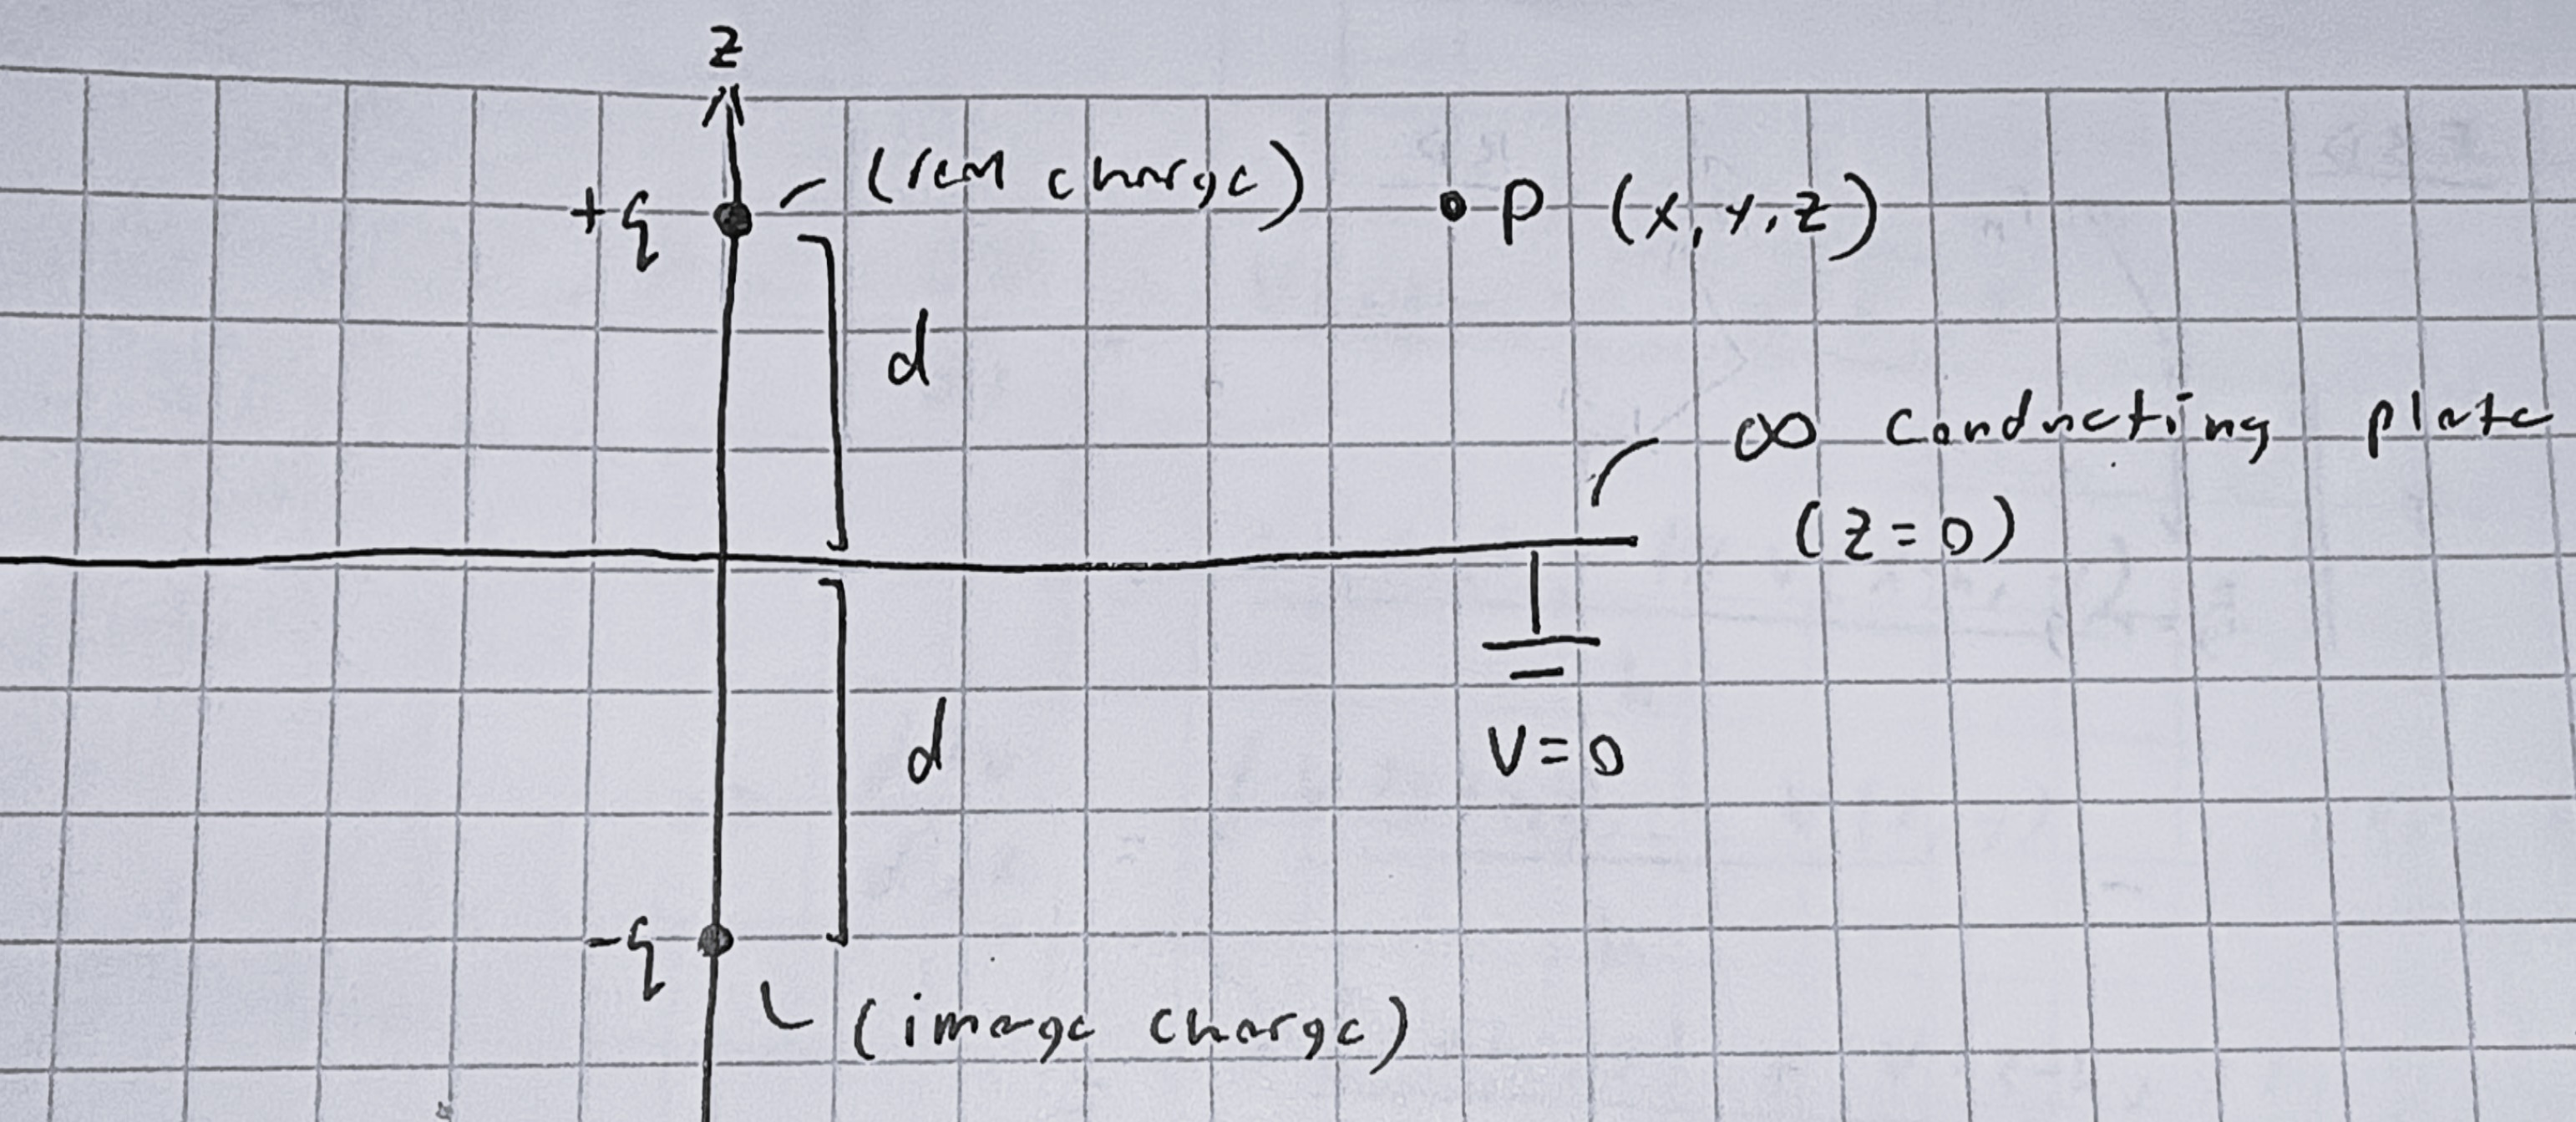
\includegraphics[width=0.8\textwidth]{method of images.JPG}
    \end{figure}
The infinite conducting plate is \textbf{grounded}:
\begin{itemize}
    \item By connecting it with a large charge reservoir (the Earth), it allows excess to charge move onto and out of the plate to maintain a zero potential.
    \item This gives us the \textbf{boundary condition} that $V=0$ over the plate.
\end{itemize}
To satisfy Laplace's equation for the region above the plate ($z>0$), we add a negative \textbf{image charge} at the mirror point $(0,0,-d)$:
\begin{itemize}
    \item This allows us to define the potential in the upper region such that as $z \to 0$, $V \to 0$. Thus satisfying the boundary condition.
\end{itemize}
\underline{Note:} To satisfy the Laplace's equation, we need a function for potential that both satisfies the boundary condition (at $z=0$) and approaches 0 as $r \to \infty$. If we didn't have the image charge, then V would go to 0 as $r \to \infty$ but it wouldn't satisfy the boundary condition.\\\\
\textbf{Finding the solution to Laplace's Equation:} (V at $P=(x,y,z)$)
\[\vec{r}_+ = \left<x,y,z\right>-\left<0,0,d\right>, \quad r=\sqrt{x^2+y^2+(z-d)^2}\]
\[\vec{r}_- = \left<x,y,z\right>-\left<0,0,-d\right> \quad r=\sqrt{x^2+y^2+(z+d)^2}\]
Thus,
\[\boxed{V_{(x,y,z)}=\frac{1}{4\pi\varepsilon_o}\left(\frac{q}{\sqrt{x^2+y^2+(z-d)^2}}-\frac{q}{\sqrt{x^2+y^2+(z+d)^2}}\right)}\]
Since is satisfies both Laplace's equation and the boundary conditions, this is the \textbf{only solution} for potential in the upper region.\\\\
Now that we have a function for potential, we can do some fun stuff such as\\\\
\textbf{Finding the z-component of electric field in the upper region}
\[E_z=-\frac{d}{dz}\left[\frac{1}{4\pi\varepsilon_o}\left(\frac{q}{\sqrt{x^2+y^2+(z-d)^2}}-\frac{q}{\sqrt{x^2+y^2+(z+d)^2}}\right)\right]\]
\[E_z = \frac{q}{4\pi\varepsilon_o}\left[\frac{(z-d)}{(x^2 + y^2 + (z-d)^2)^{3/2}}
- \frac{(z+d)}{(x^2 + y^2 + (z+d)^2)^{3/2}}\right]\]
Since we know that the electric field near a conductor is normal to the surface with magnitude $E=\sigma/\varepsilon_o$, we can \\\\
\textbf{Find the surface charge density of the conducting plate}
\[E_z(z=0)=\frac{q}{4\pi\varepsilon_o}\left[\frac{-d}{(x^2 + y^2 + d^2)^{3/2}}
- \frac{d}{(x^2 + y^2 + d^2)^{3/2}}\right]\]
Thus,
\[\sigma(x,y,z=0)=\frac{-2qd}{4\pi(x^2+y^2+d^2)^{3/2}}\]
\underline{Note:} We can check our results by integrating
\[\int_{-\infty}^{\infty}\int_{-\infty}^{\infty}\sigma dxdy=-q\]
    \item Use the ``relaxation'' method to numerically solve for the electric potential outside of a conductor held at a fixed potential.\\\\
Our goal is to solve Laplace's equation by evaluating derivatives at discrete points using the Finite Difference Method.
\[\nabla^2V=\frac{d^2V}{dx^2}+\frac{d^2V}{dy^2}=0\]
\textbf{Set up:} $P=(x,y)$
\begin{figure}[H]
            \centering
            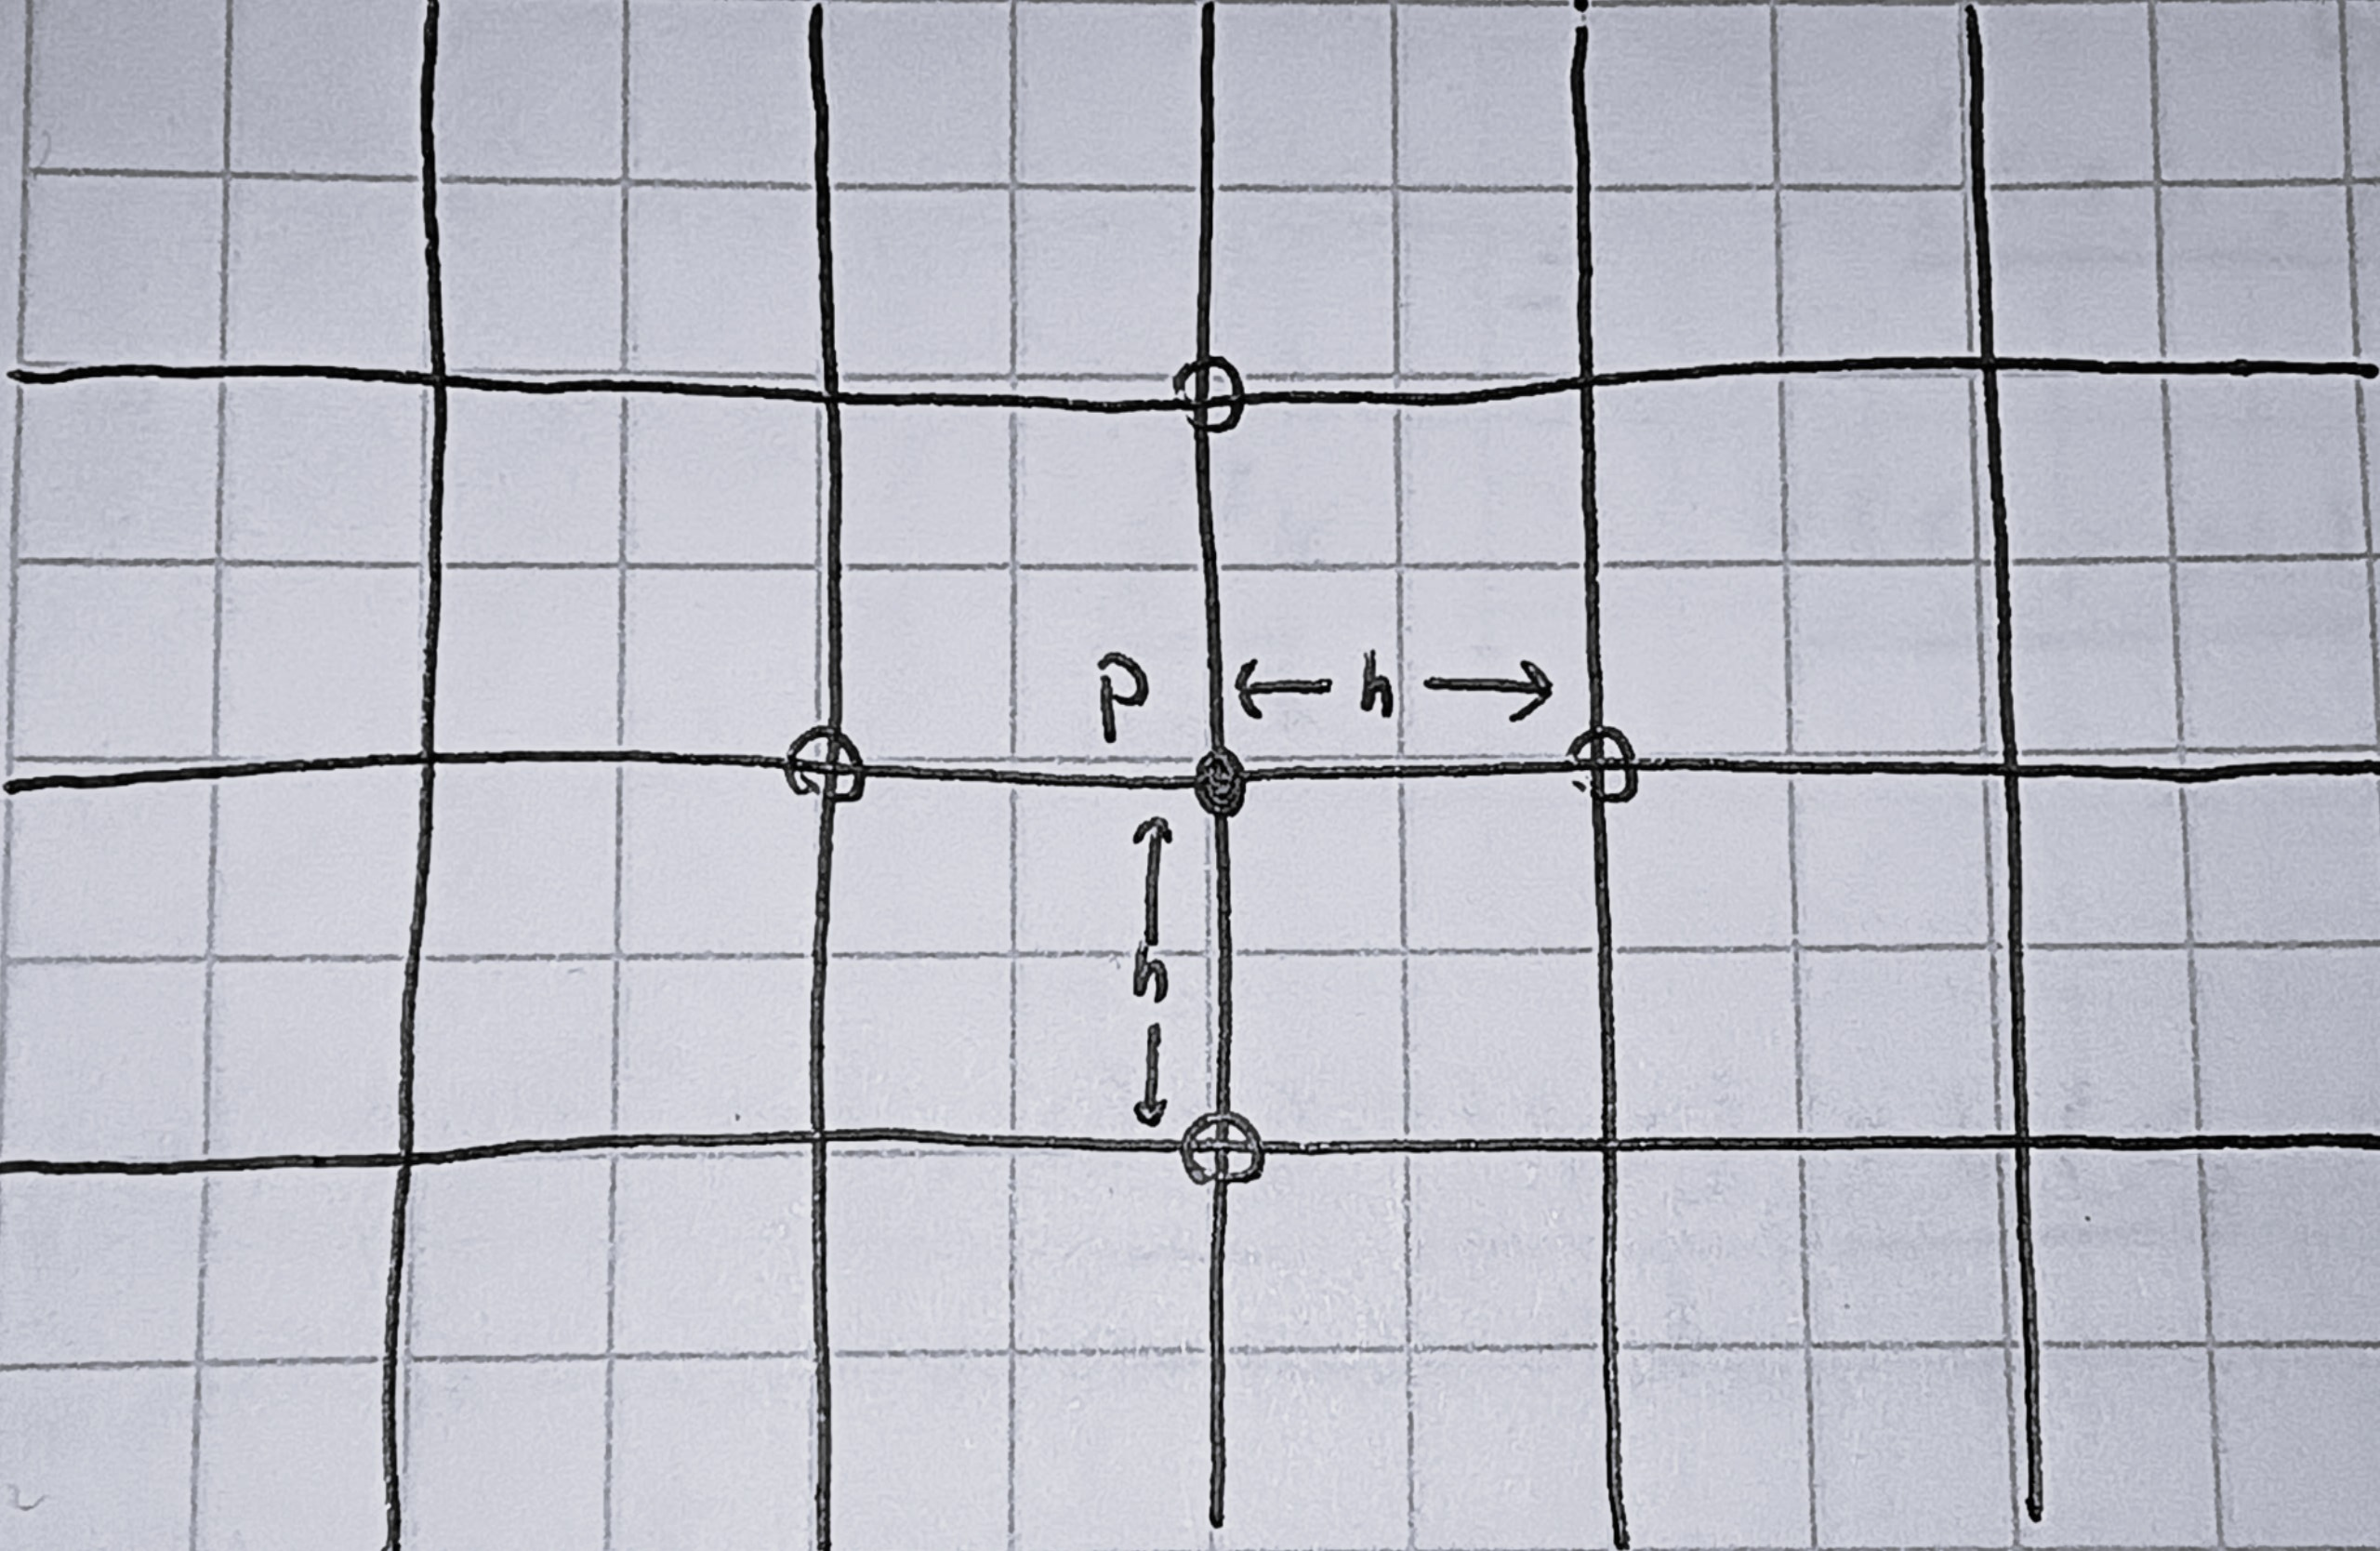
\includegraphics[width=0.5\textwidth]{relaxxx.JPG}
    \end{figure}
\end{enumerate}
Evaluating Laplace's equation locally at P:
\[\frac{dV}{dx}=\frac{V(x+h,y)-V(x,y)}{h}=\frac{V(x,y)-V(x-h,y)}{h}\]
\underline{Note:} These are the forward and backward first-differences for the derivative.
\begin{align*}
    \frac{d^2V}{dx^2}=&\frac{\left(\frac{V(x+h,y)-V(x,y)}{h}\right)-\left(\frac{V(x,y)-V(x-h,y)}{h}\right)}{h}\\
    =&\frac{V(x+h,y)+V(x-h,y)-2V(x,y)}{h^2}
\end{align*}
Similarly,
\[\frac{d^2V}{dy^2}=\frac{V(x,y+h)+V(x,y-h)-2V(x,y)}{h^2}\]
Plugging into Laplace's Equation we get:
\[\boxed{V(x,y)=\frac{1}{4}\left[V(x+h,y)+V(x-h,y)+V(x,y+h)+V(x,y-h)\right]}\]
In other words, the potential at P is the average of the potentials at its 4 adjacent points.\\\\
The \textbf{Relaxation Method} essentially calculates potentials at every point (not on the boundary) and iterates using previously calculated values until it converges. 

\section*{Chapter 25 - Capacitance}
\begin{enumerate}
    \item Define the capacitance and explain its utility.
    \item Calculate the capacitance for various arrangements of conductors. Especially be familiar with the properties of the ideal parallel plate capacitor.
    \item Explain the use of dielectrics, their physics principles, and calculate capacitance in the presence of dielectric materials.
    \item Derive the electric field energy density. Calculate the electrostatic energy stored in a capacitor several different ways i.e., using expressions that directly involve the capacitance or computing the volume integral over the electric field energy density.
\end{enumerate}
\section*{Chapter 26 - Current and Resistance}
\begin{enumerate}
    \item Define resistance and know Ohm's law. Use it to find the electric field in and potential difference across a resistor.
    \item Know the relations among power, potential, and resistance. Calculate the power dissipated in a resistor.
\end{enumerate}
\textbf{End Exam 2}
sasses  
\end{document}